\documentclass[12pt,a4paper,onecolumn]{article}
\usepackage{paralist}
\usepackage{indentfirst}
%\usepackage[numbers,sort\ & compress]{natbib}
\usepackage[top=1.5cm,bottom=1.5cm,left=3cm,right=3cm]{geometry} %页边距包
\usepackage{amsmath}
\usepackage{flushend,cuted}
\usepackage{caption}
\usepackage{subcaption}
\usepackage{ctex}
\usepackage{float} %控制图像固定
\usepackage{listings} %代码
\usepackage{color}
\definecolor{mygreen}{rgb}{0,0.6,0}
\definecolor{mygray}{rgb}{0.5,0.5,0.5}
\definecolor{mymauve}{rgb}{0.58,0,0.82}
\lstset{ %
	backgroundcolor=\color{white},   % choose the background color; you must add \usepackage{color} or \usepackage{xcolor}
	basicstyle=\footnotesize,        % the size of the fonts that are used for the code
	breakatwhitespace=false,         % sets if automatic breaks should only happen at whitespace
	breaklines=true,                 % sets automatic line breaking
	captionpos=b,                    % sets the caption-position to bottom
	commentstyle=\color{mygreen},    % comment style
	deletekeywords={...},            % if you want to delete keywords from the given language
	escapeinside={\%*}{*)},          % if you want to add LaTeX within your code
	extendedchars=true,              % lets you use non-ASCII characters; for 8-bits encodings only, does not work with UTF-8
	%frame=single,	                   % adds a frame around the code
	keepspaces=true,                 % keeps spaces in text, useful for keeping indentation of code (possibly needs columns=flexible)
	keywordstyle=\color{blue},       % keyword style
	language=R,                 % the language of the code
	otherkeywords={*,...},           % if you want to add more keywords to the set
	numbers=left,                    % where to put the line-numbers; possible values are (none, left, right)
	numbersep=5pt,                   % how far the line-numbers are from the code
	numberstyle=\tiny\color{mygray}, % the style that is used for the line-numbers
	rulecolor=\color{black},         % if not set, the frame-color may be changed on line-breaks within not-black text (e.g. comments (green here))
	showspaces=false,                % show spaces everywhere adding particular underscores; it overrides 'showstringspaces'
	showstringspaces=false,          % underline spaces within strings only
	showtabs=false,                  % show tabs within strings adding particular underscores
	stepnumber=1,                    % the step between two line-numbers. If it's 1, each line will be numbered
	stringstyle=\color{mymauve},     % string literal style
	tabsize=2,	                   % sets default tabsize to 2 spaces
	%title=\lstname                   % show the filename of files included with \lstinputlisting; also try caption instead of title
}
%\usepackage{fancyhdr} %控制页眉
%\renewcommand\refname{参考文献}
%\newcommand{\upcite}[1]{\textsuperscript{\textsuperscript{\cite{#1}}}}
\linespread{1.2}

\begin{document}
\captionsetup[figure]{name={图}}
\captionsetup[table]{name={表}}

\begin{center}
\begin{Huge}
\textbf{英超球员数据分析}
\end{Huge}
\vskip 15mm
\end{center}

\section{研究目的}

我们希望通过分析英超球员上一年的数据,对球员进行综合评价,并探索何时的方法预测球员下一年的进球数量。本文在综合评价中使用了因子分析的研究方法,在预测球员下一年进球数量时,使用了基于lasso算法的伯努利回归。

\section{数据结构}

原始数据包含了英超15只球队167名队员某年的所有数据,数据结构如下所示:

\begin{table}[H]
\centering
\caption{数据字段和解释}
\begin{tabular}{cccccc}
  \hline
    字段 & 数据类型 & 单位 & 字段 & 数据类型 & 单位\\\hline
    球员 & character & 无 & 球队 & character & 无 \\
    号码 & character & 无  & 位置 & character & 无 \\
    出场 & integer & 次数 & 首发 & integer & 次数 \\
    出场时间 & integer & 元  & 进球 & integer & 次数 \\
    助攻 & integer & 次数  & 传球 & integer & 次数 \\
    过人 & integer & 次数  & 抢断 & integer & 次数 \\
    越位 & integer & 次数  & 犯规 & integer & 次数 \\
    红牌 & integer & 次数  & 黄牌 & integer & 次数 \\
    射门 & integer & 次数 & 射正 & integer & 次数 \\
		射门成功率 & numeric & 比例 & 头球进球 & integer & 次数 \\
    左脚进球 & integer & 次数 & 右脚进球 & integer & 次数 \\
    直接任意球进球 & integer & 次数 & 点球 & integer & 次数 \\
    赢得点球机会 & integer & 次数 & 拦截 & integer & 次数 \\
    解围 & integer & 次数 & 头球解围 & integer & 次数 \\
    头球争顶成功 & integer & 次数 & 乌龙球 & integer & 次数 \\
 下一年进球 & integer & 次数 & & & \\
    \hline
  \end{tabular}
\end{table}

\section{因子分析}

\subsection{协方差矩阵}

因子分析模型适用于变量之间存在相关关系的数据,对于我们的数据,变量之间是否存在相关关系呢?我们可以通过协方差矩阵进行检验。如下是我们数据的协方差矩阵图:

\begin{figure}[H]
\centering
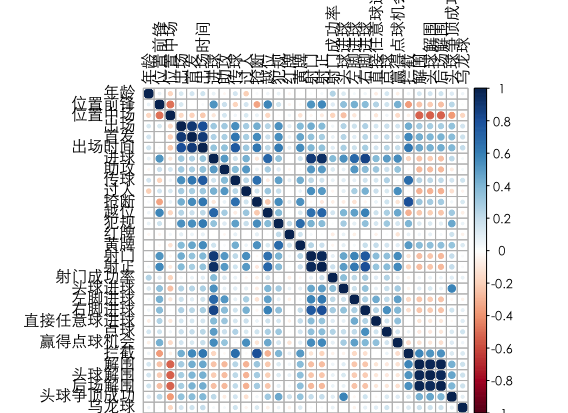
\includegraphics[width=400pt]{协方差矩阵.png}
\caption{\small{协方差矩阵}}
\end{figure}

由上图可知,虽然我们的数据变量很多,但是在这些变量中,有很多变量是显著正相关的。这就提醒我们应该采取适当的降维方法。同时,我们观察到,变量之间的相关关系似乎可以分成三块,第一块对应球员的进攻能力,第二块对应球员的辅助能力,第三块对应球员的防守能力。这就提醒我们可以采取因子分析的方法,尝试提取出这几个因子代表全部的变量信息。

\subsection{提取主成分}

提取数据的主成分并输出所有主成分的标准差、方差贡献率和方差累计贡献率。

\begin{table}[H]
\centering
\caption{主成分分析}
\begin{tabular}{ccccccc}
  \hline
     & 成分一 & 成分二 & 成分三 & 成分四 & 成分五 & 成分六 \\\hline
    标准差 & 2.80 & 2.50 & 1.72 & 1.27 & 1.23 & 1.07 \\
    方差贡献率 & 26.2\% & 21.0\% & 10.0\% & 5.4\% & 5.0\% & 3.8\% \\
    方差累计贡献率 & 26.2\% & 47.2\% & 57.2\% & 62.6\% & 67.6\% & 71.4\% \\
    \hline
  \end{tabular}
\end{table}

\begin{figure}[H]
\centering
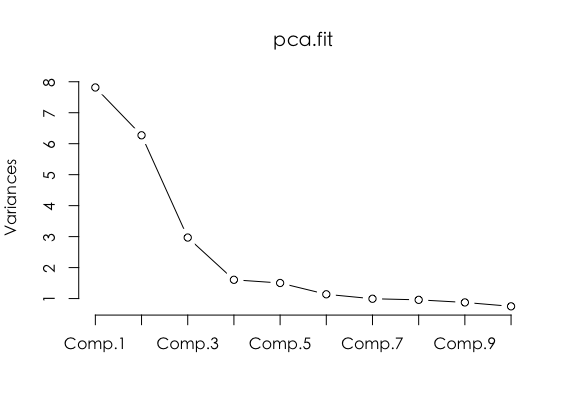
\includegraphics[width=400pt]{碎石图.png}
\caption{\small{碎石图}}
\end{figure}

如上图表所示,前六个主成分的方差累计贡献率已经超过了70\%,可以认为前六个主成分已经提取了原始数据中的大部分信息。所以本文的分析就使用六个因子的因子分析。

\subsection{提取公因子}

本文提取公因子的方法为主成分方差最大旋转法。通过方差最大旋转之后,公因子的标准差、方差贡献率和累计方差贡献率如下:

\begin{table}[H]
\centering
\caption{因子分析}
\begin{tabular}{ccccccc}
  \hline
     & 因子一 & 因子二 & 因子三 & 因子四 & 因子五 & 因子六 \\\hline
    标准差 & 7.0 & 5.4 & 3.9 & 1.9 & 1.8 & 1.3 \\
    方差贡献率 & 23.4\% & 18.1\% & 13.1\% & 6.4\% & 6.0\% & 4.5\% \\
    方差累计贡献率 & 23.4\% & 41.5\% & 54.6\% & 61.0\% & 67.0\% & 71.0\% \\
    \hline
  \end{tabular}
\end{table}

这六个公因子的累计贡献率也大于了70\%。说明我们提取公因子的方法是合理的。现在我们要对这六个公因子做解释。

我们可以使用分析因子载荷阵的方法分析每个公因子的含义。因子载荷阵在附录中给出。

因子载荷阵的结果显示,第一因子解释为进攻因子、第二因子解释为辅助因子、第三因子解释为防守因子、第四因子解释为犯规因子、第五因子解释为准确度因子、第六因子解释为任意球因子。

以第一公因子为横轴,第二公因子为纵轴,将所有球员的数据绘制成散点图展示如图。

\begin{figure}[H]
\centering
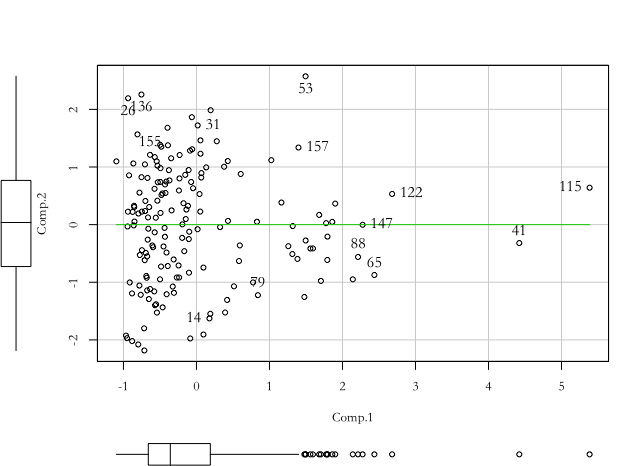
\includegraphics[width=400pt]{两个公因子.png}
\caption{\small{因子分析图}}
\end{figure}

我们可以在图中标记出第一公因子或者第二公因子较大的几个点坐标,这些点是115、41、122、147、157、53、31、36.我找到了这些球员分别是苏亚雷斯、范佩西、马塔、本特克、阿扎尔、卡索拉、皮纳尔、科尔。这些球员的确是英超联赛中表现比较优秀的球员。

\subsection{综合评价}

现在我们已经得到了每个球员的六个因子得分,现在我们可以用因子分析对每个球员进行综合评价。我采取的可视化方法是绘制不同球员的风玫瑰图来从六个维度比较不同球员的能力。我筛选了进攻因子、辅助因子和防守因子排名在前4的所有球员绘制了风玫瑰图如下。

\begin{figure}[H]
\centering
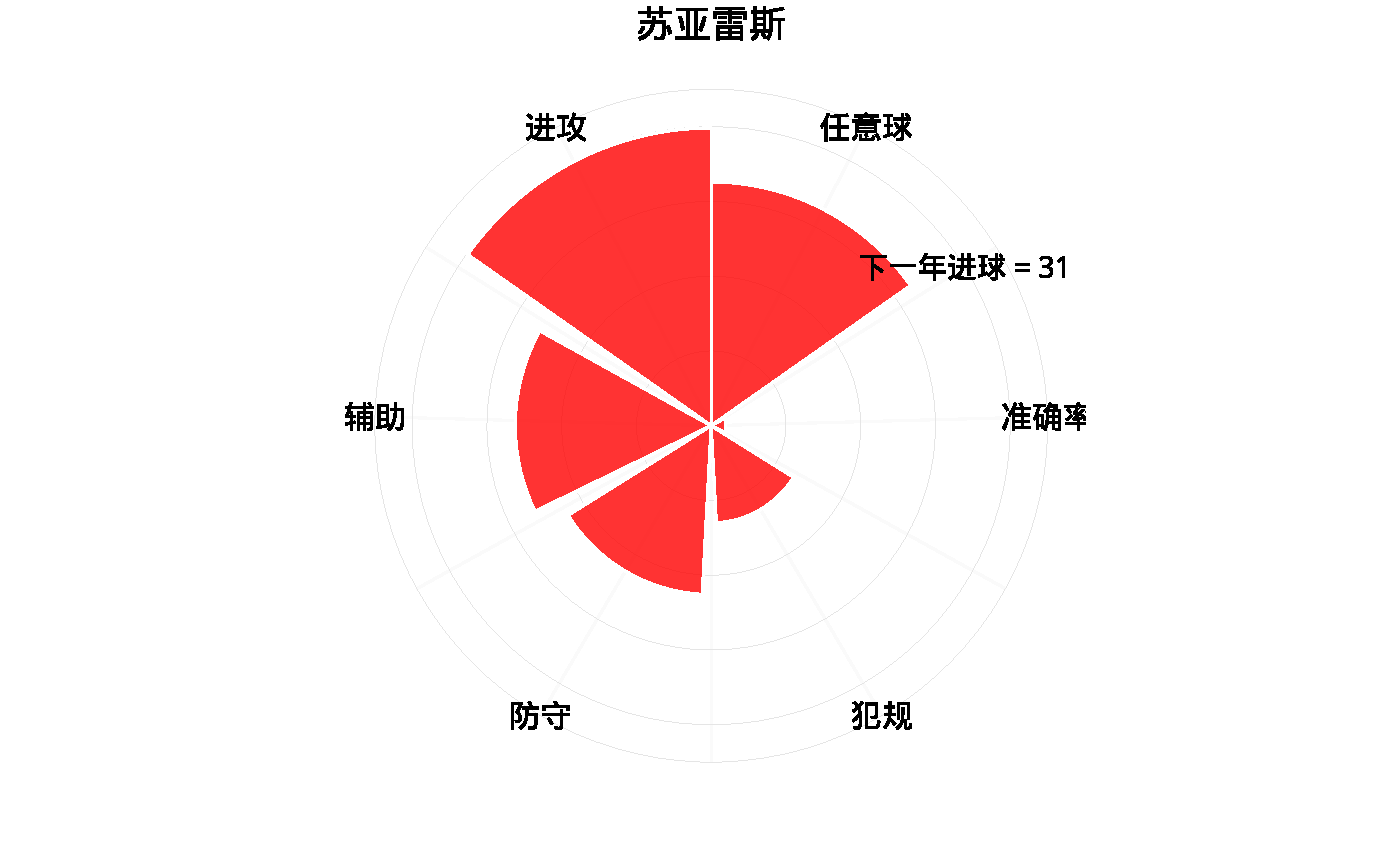
\includegraphics[width=100pt]{前锋苏亚雷斯.pdf}
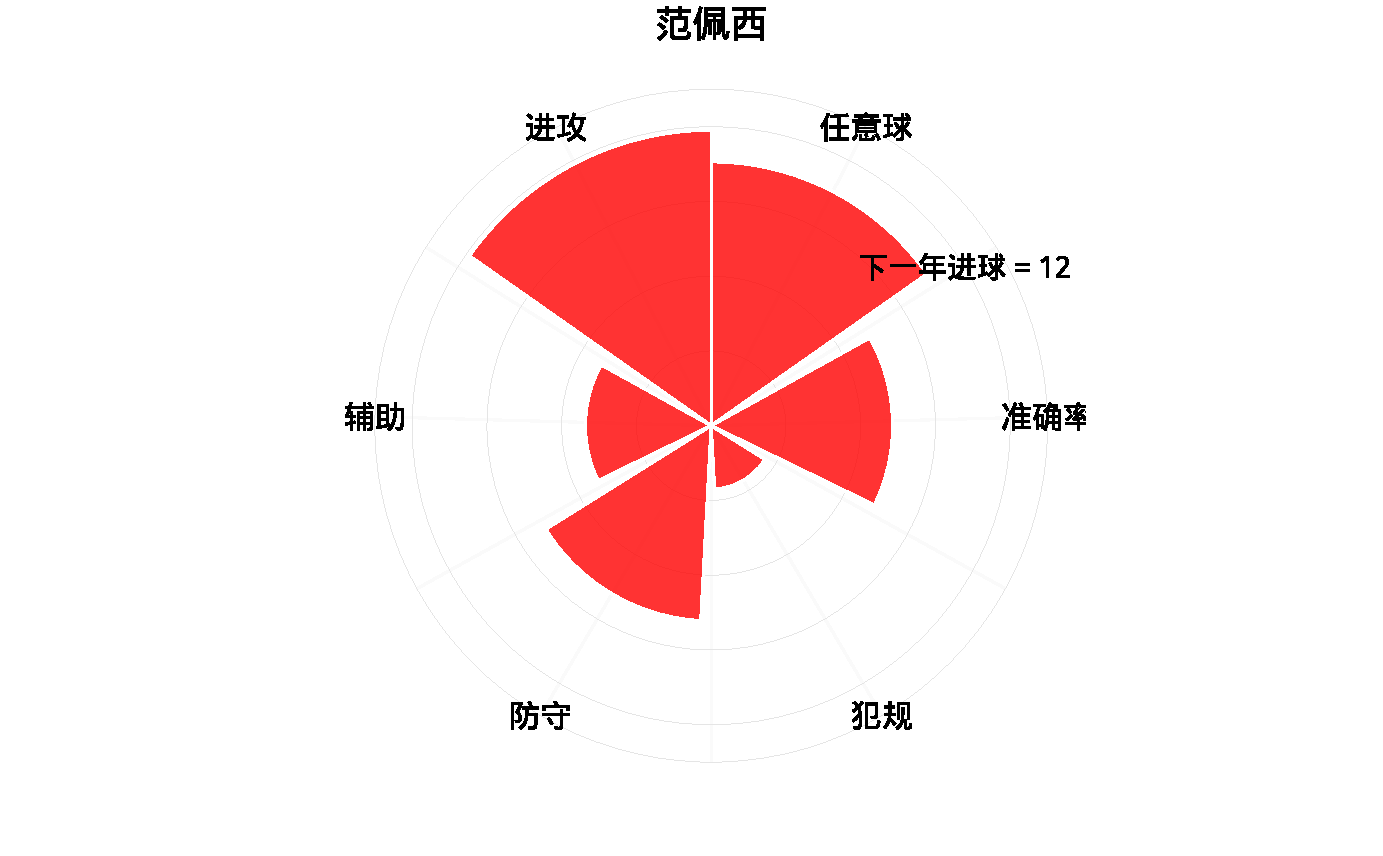
\includegraphics[width=100pt]{前锋范佩西.pdf}
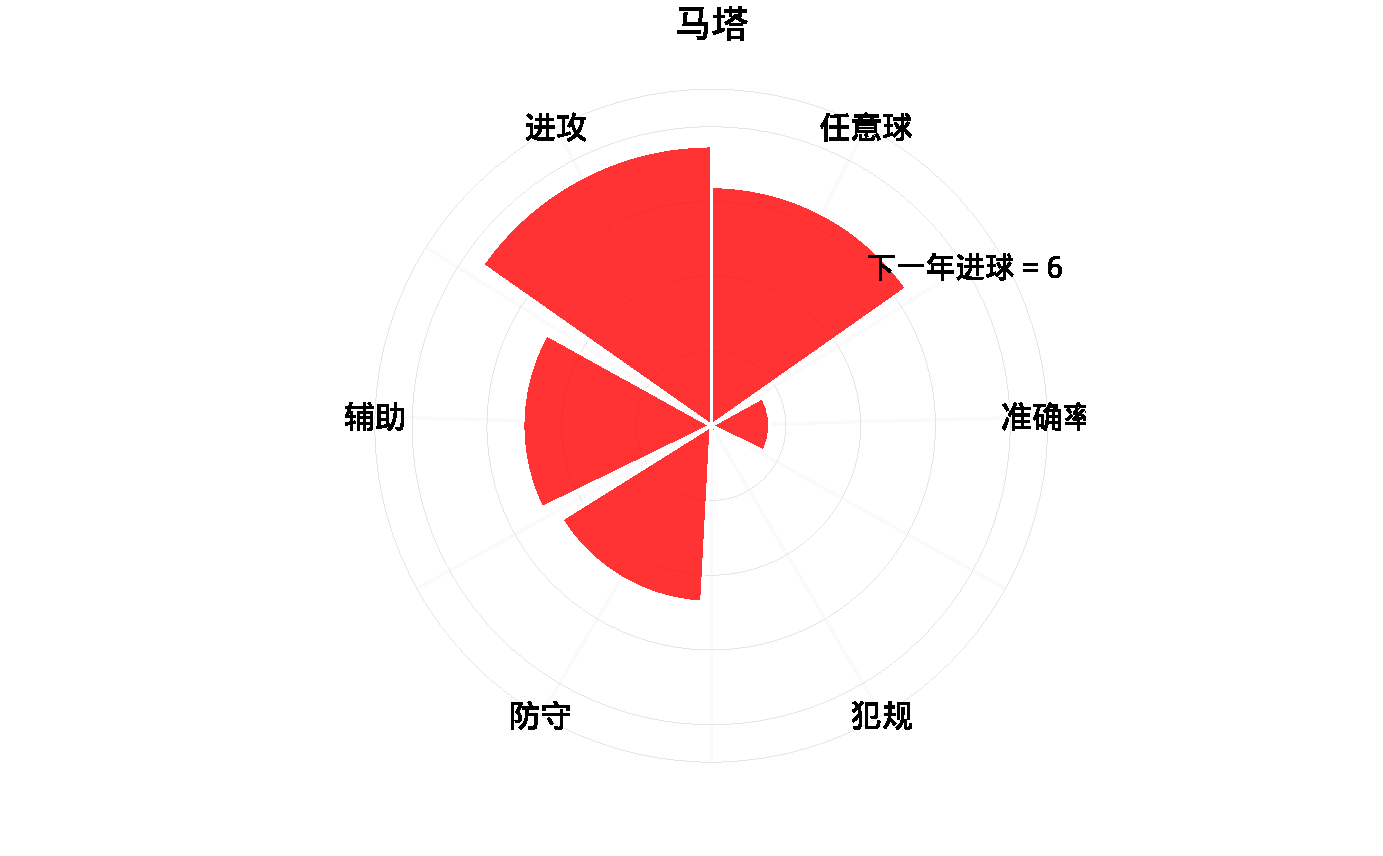
\includegraphics[width=100pt]{前锋马塔.pdf}
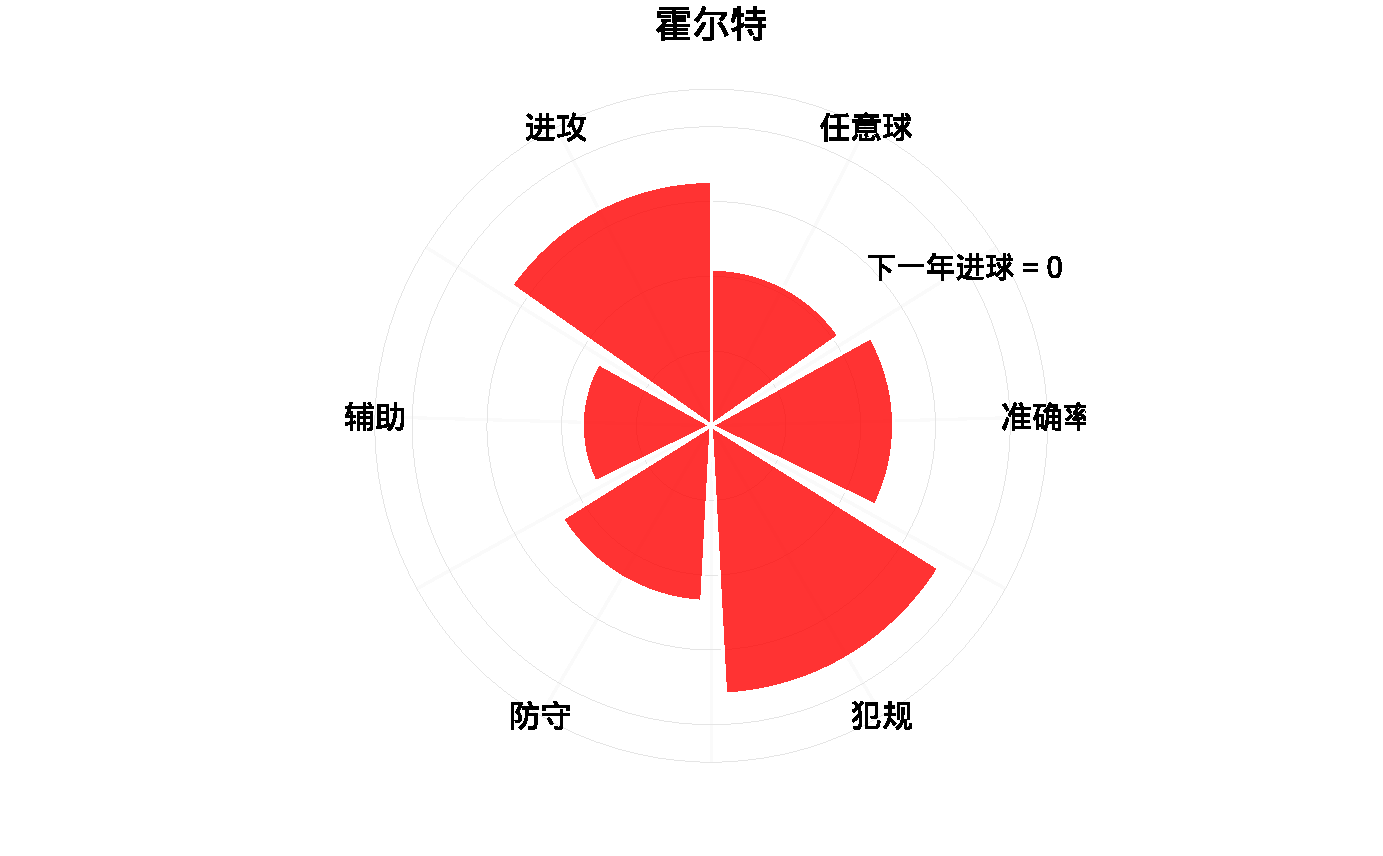
\includegraphics[width=100pt]{前锋霍尔特.pdf}
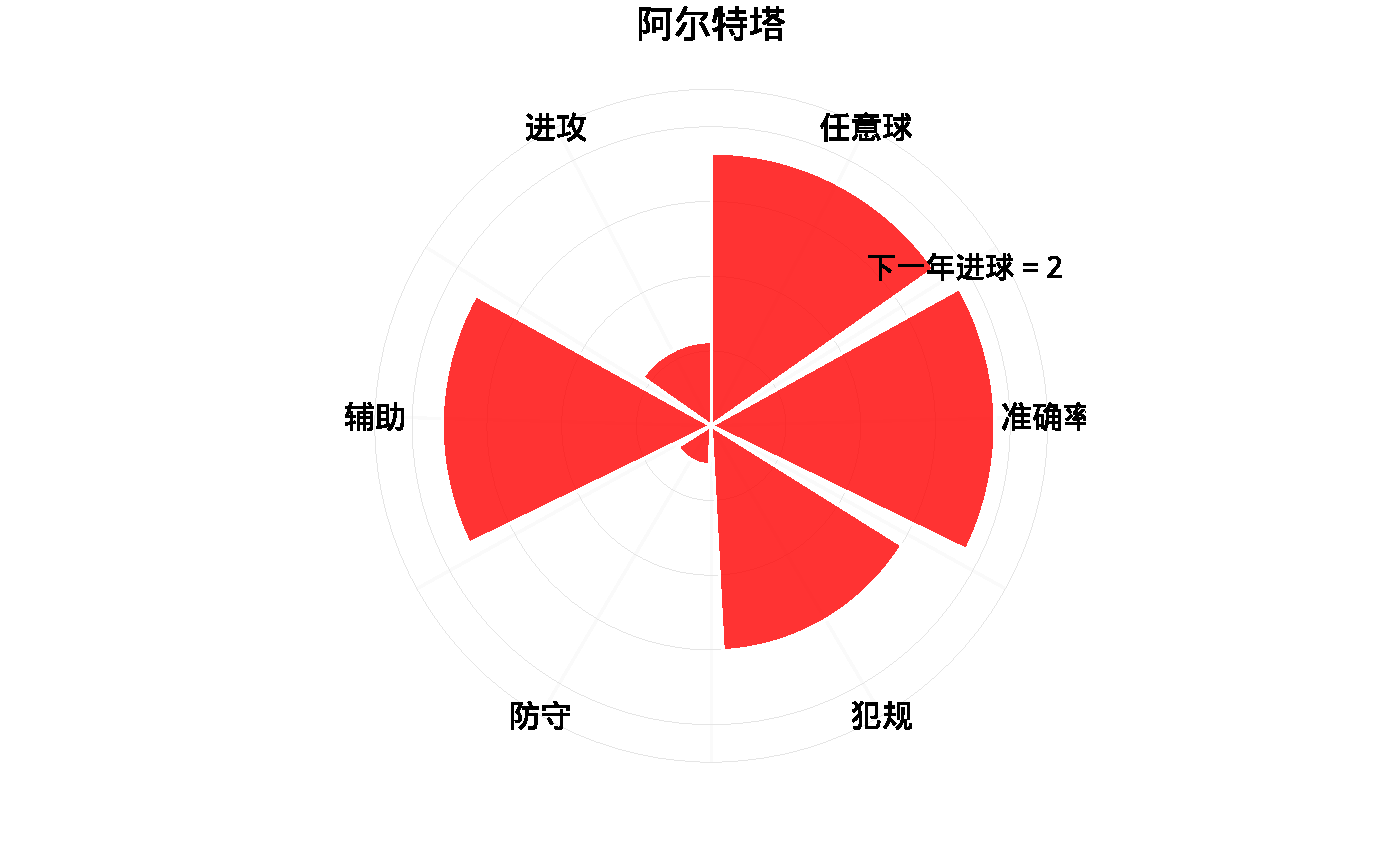
\includegraphics[width=100pt]{中场阿尔特塔.pdf}
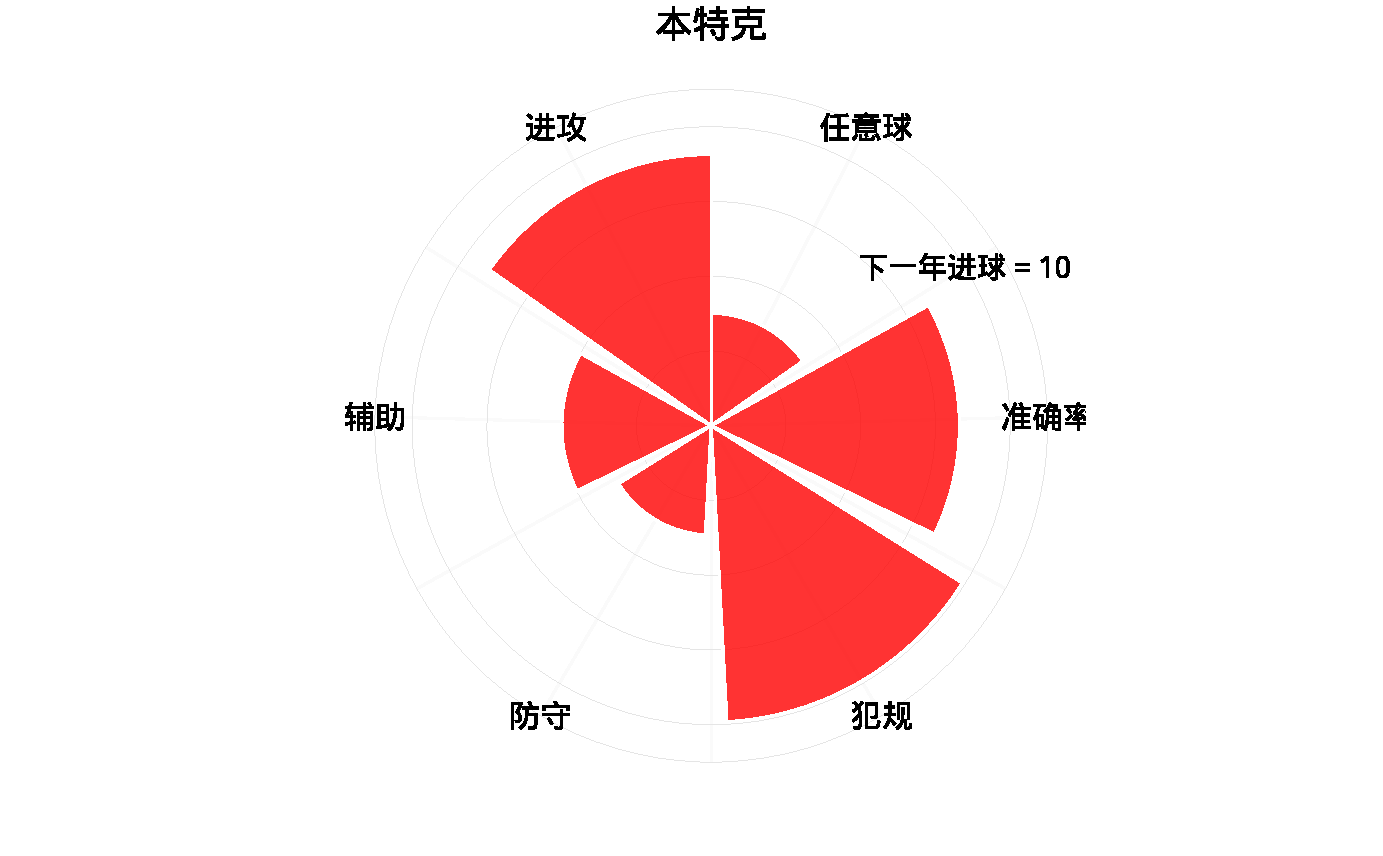
\includegraphics[width=100pt]{中场本特克.pdf}
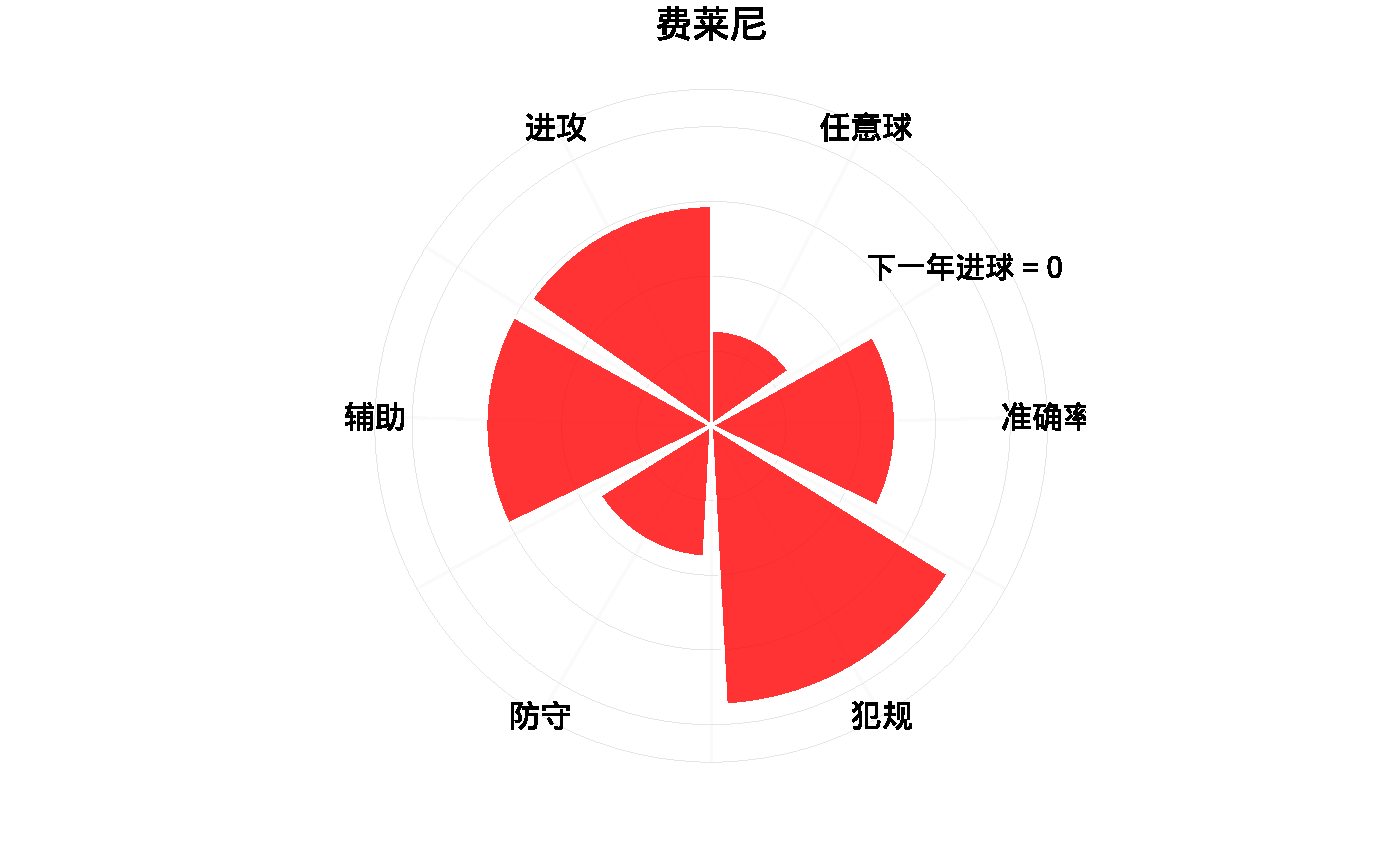
\includegraphics[width=100pt]{中场费莱尼.pdf}
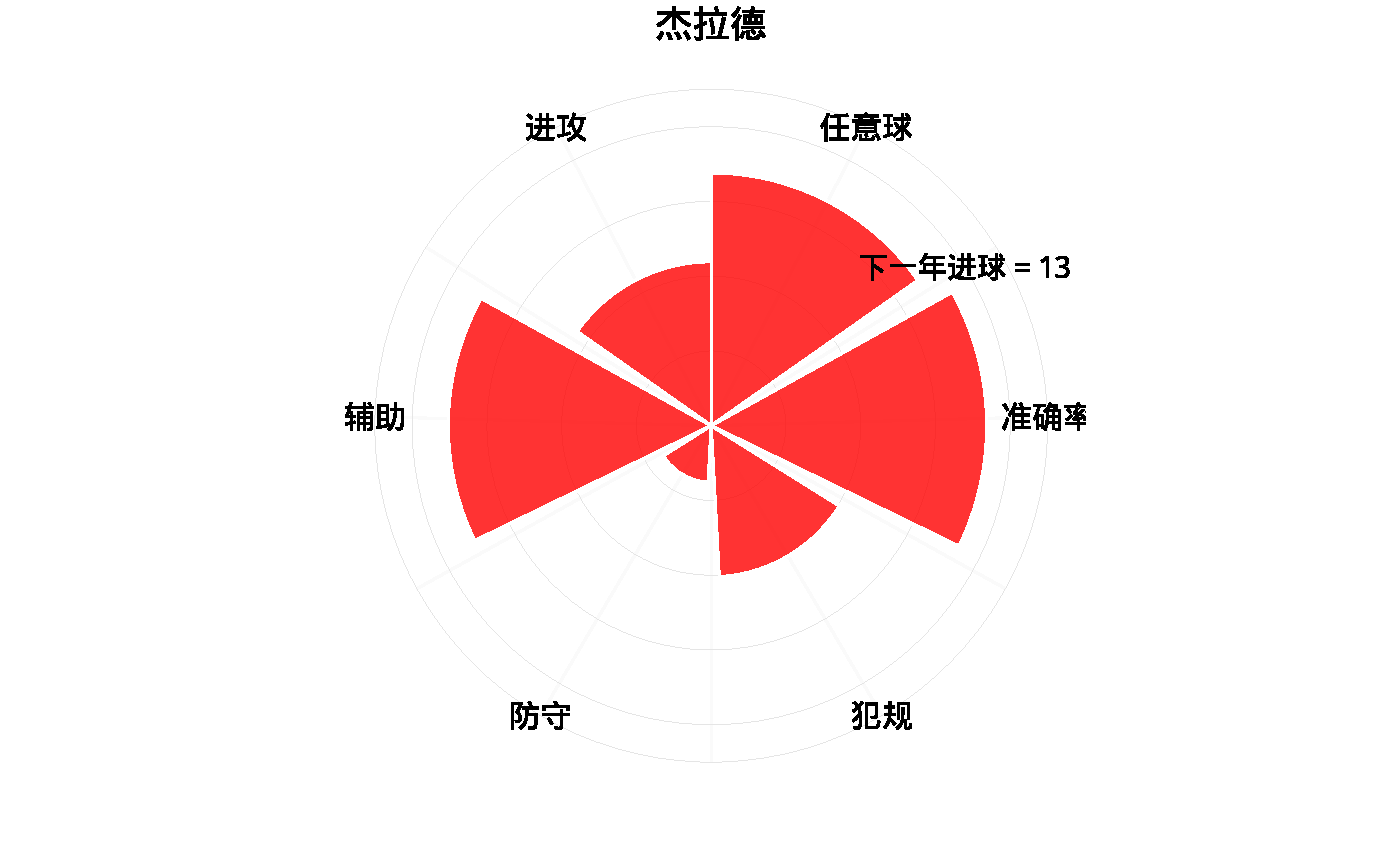
\includegraphics[width=100pt]{中场杰拉德.pdf}
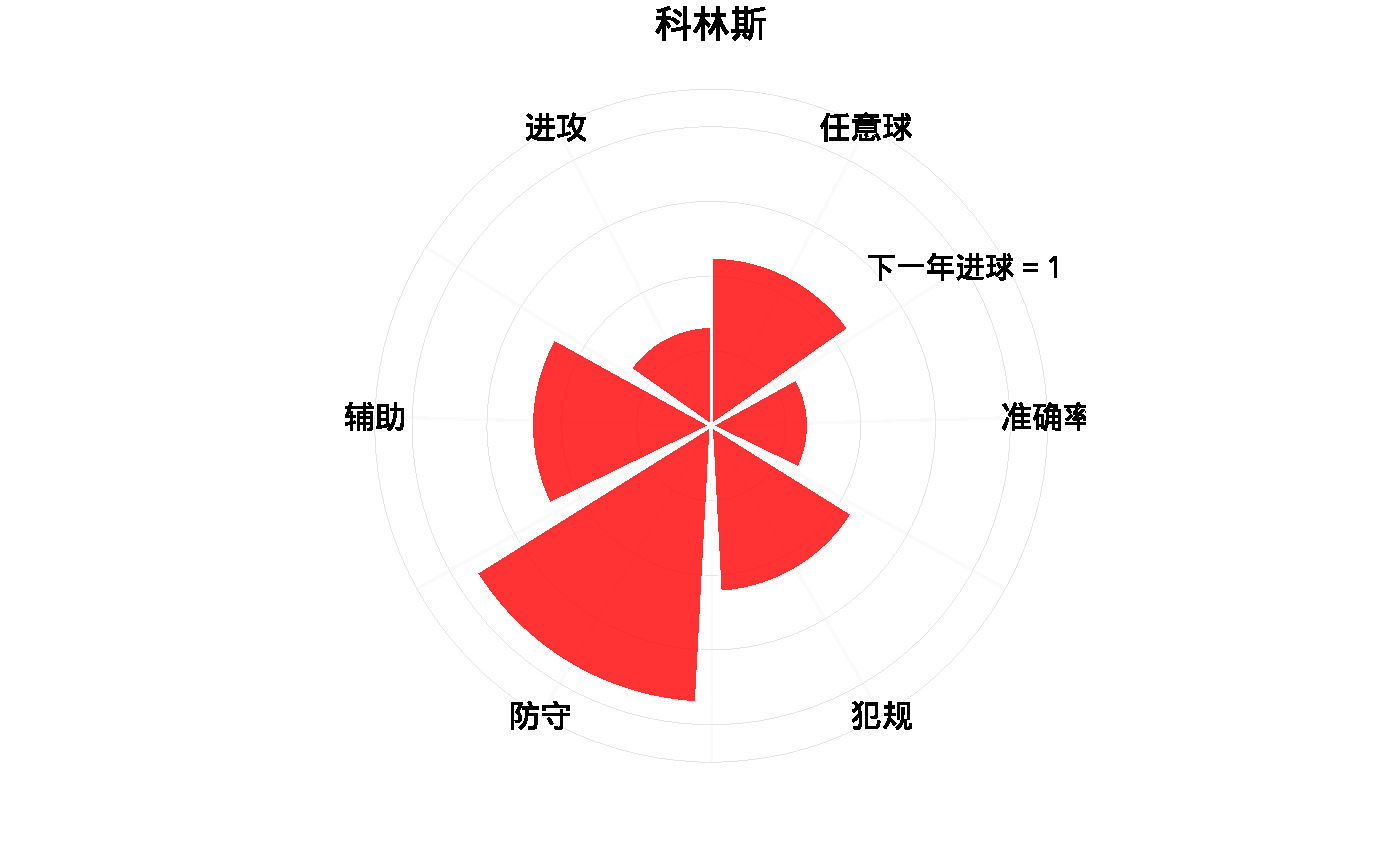
\includegraphics[width=100pt]{后卫科林斯.pdf}
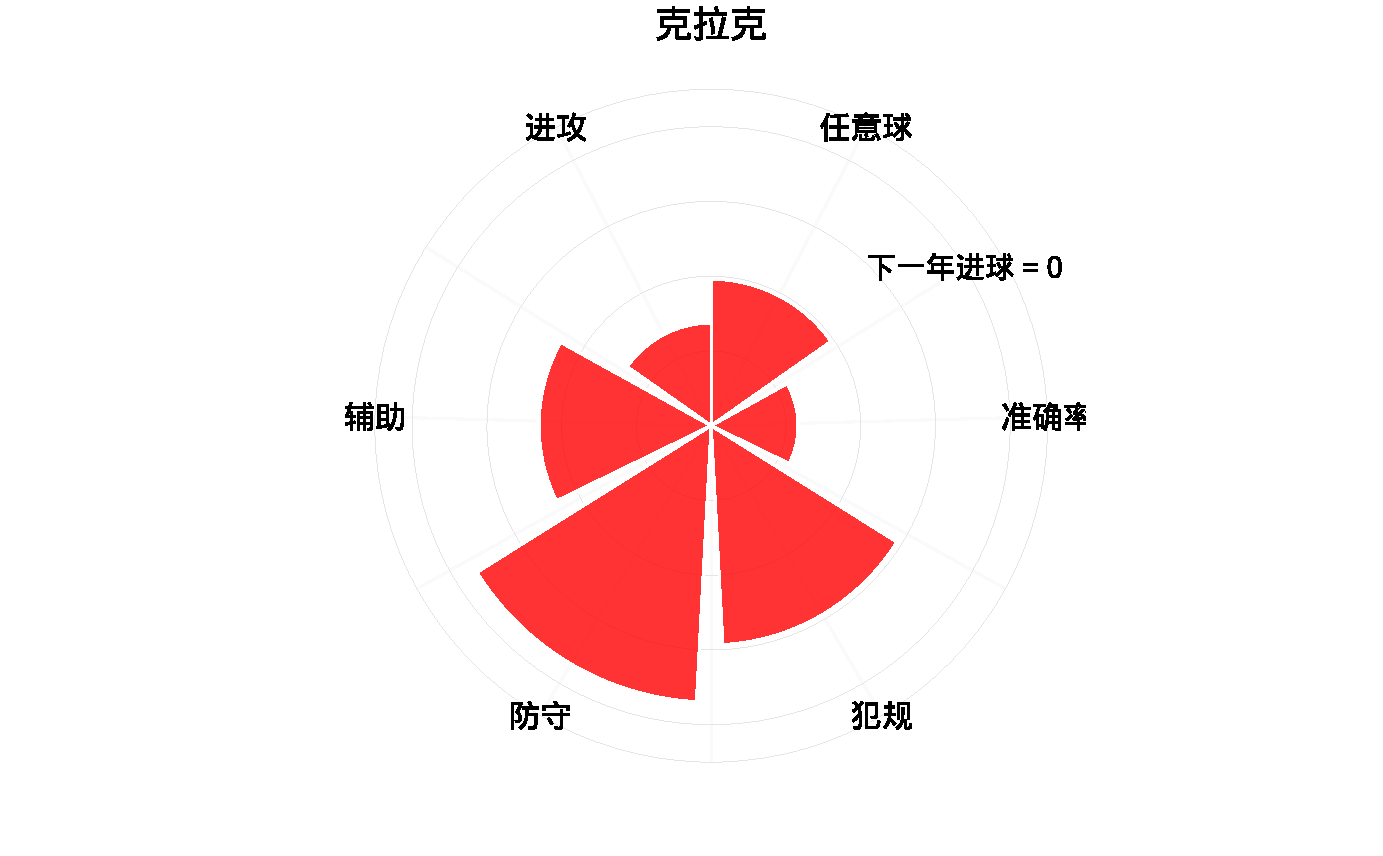
\includegraphics[width=100pt]{后卫克拉克.pdf}
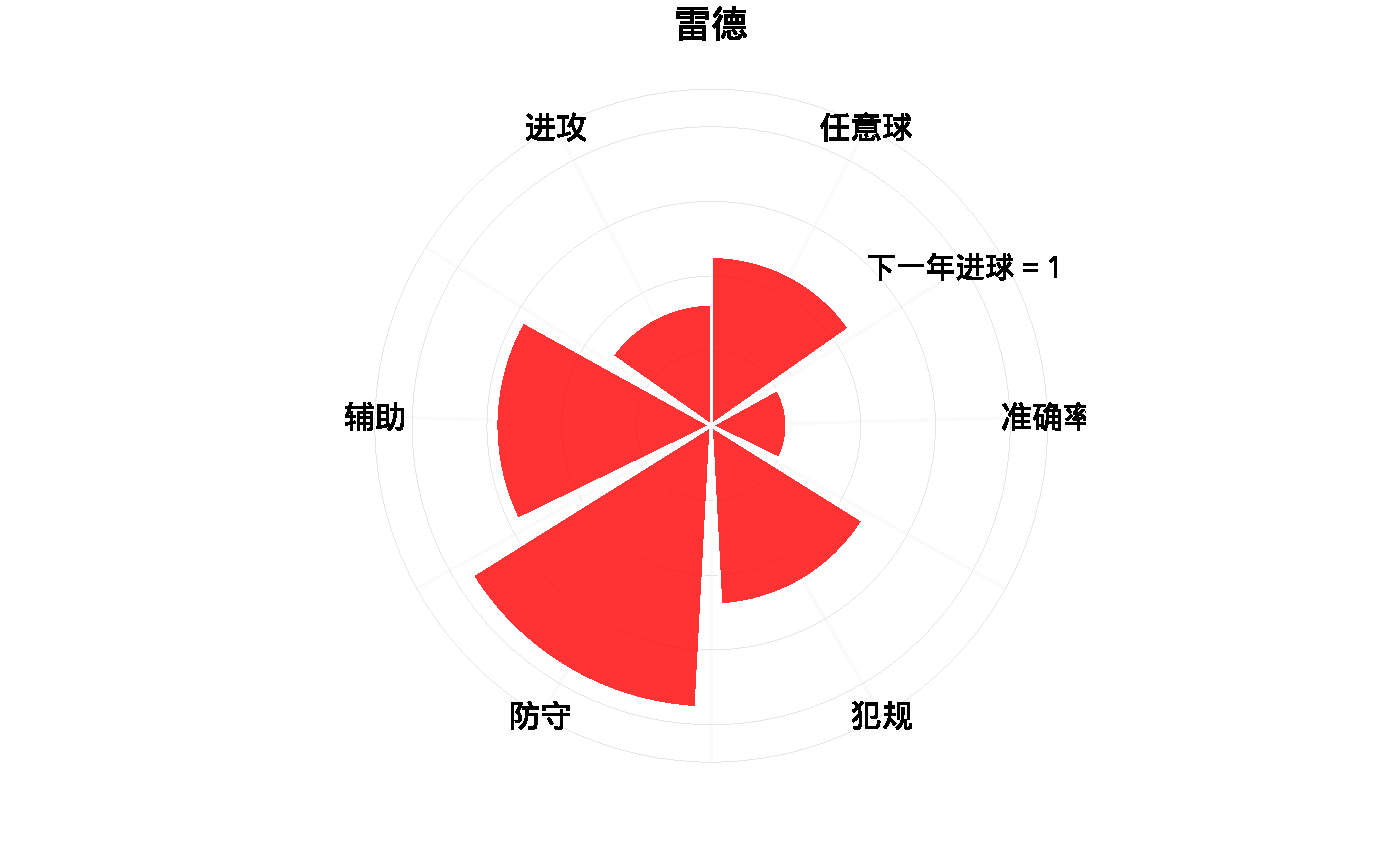
\includegraphics[width=100pt]{后卫雷德.pdf}
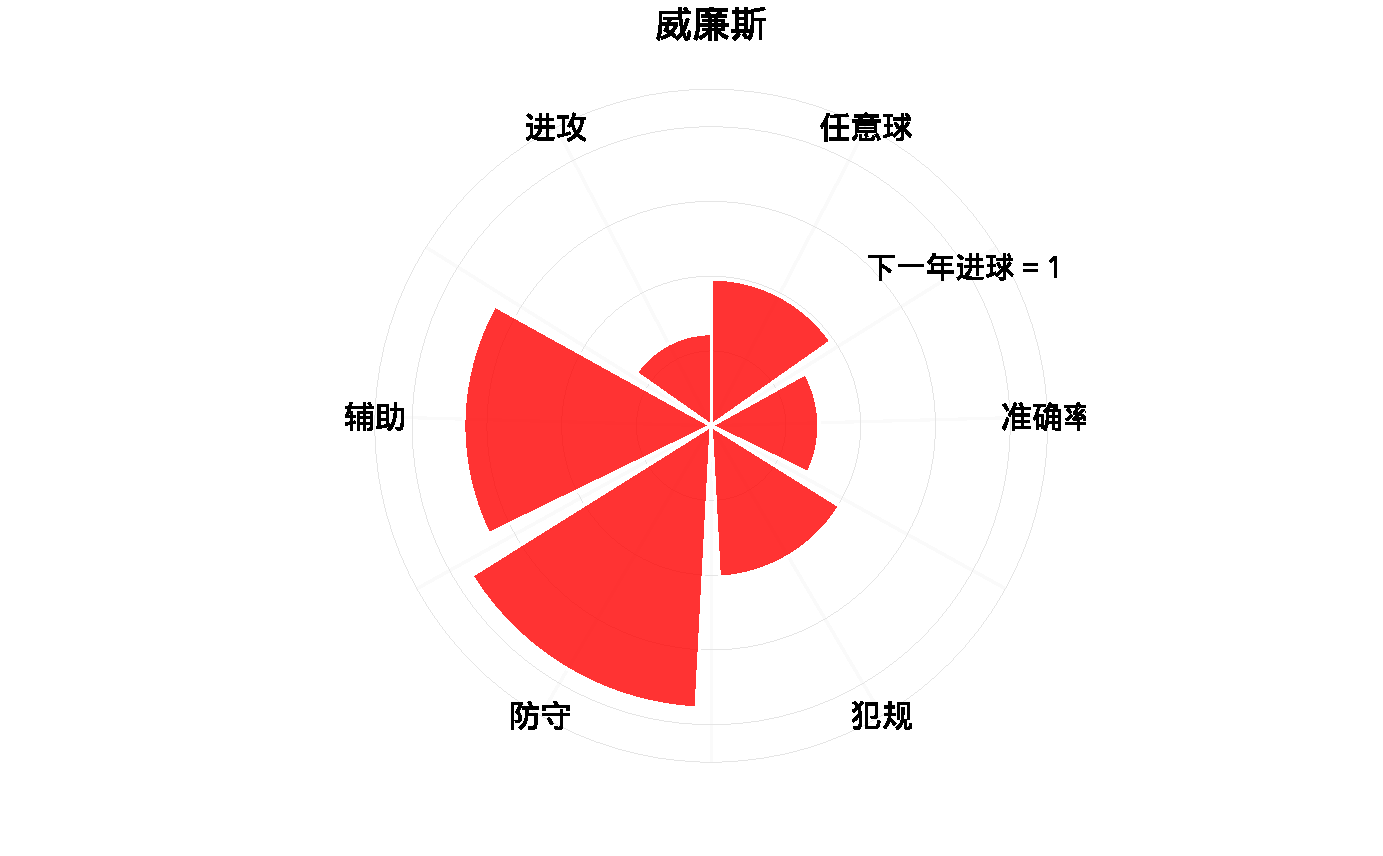
\includegraphics[width=100pt]{后卫威廉斯.pdf}
\caption{\small{不同球员之间的比较}}
\end{figure}

上图第一列表示进攻因子排名靠前的球员、第二列表示辅助因子排名靠前的球员、第三列表示防守因子排名靠前的球员。查找资料之后可知,这三列对应着英超联赛中优秀的前锋球员、中场球员和后卫球员。说明我们的方法对评价英超球员的个人能力是真实的,有参考的价值。

\section{预测英超球员下一年进球}

本文假设进球数量服从伯努利分布,所有我们可以采取广义线性模型中的伯努利回归对英超球员数据做回归分析。

我首先做了全变量的回归分析,全变量的回归分析之后的参数如下所示:

\begin{table}[H]
\centering
\caption{回归分析}
\begin{tabular}{cccccc}
  \hline
	变量 &参数 &p值 &变量 &参数 &p值 \\\hline
 (Intercept) & 0.59942 & 2e-16 & 年龄 & -0.27098 & 1.44e-05\\
 位置前锋 & 0.52450 & 0.000119 & 位置中场 & 0.32712 & 0.049891\\
 出场 & 0.15583 & 0.198599 & 首发 & 0.15462 & 0.288706\\
 出场时间 & -0.62097 & 0.000568 & 进球 & -2.16405 & 0.446019\\
 助攻 & 0.01144 & 0.844174 & 传球 & 0.47245 & 7.47e-07\\
 过人 & 0.13921 & 0.041716 & 抢断 & 0.15657 & 0.192480\\
 越位 & -0.22079 & 0.006452 & 犯规 & 0.02145 & 0.834742\\
 红牌 & 0.08655 & 0.110416 & 黄牌 & 0.11760 & 0.135630\\
 射门 & 0.24199 & 0.316336 & 射正 & 0.08289 & 0.767087\\
 射门成功率 & 0.04115 & 0.690152 & 头球进球 & 0.44887 &0.499551  \\
 左脚进球 & 1.27367 & 0.347323 & 右脚进球 & 1.54170 & 0.389795    \\
 直接任意球进球 & -0.16616 & 0.001101 & 点球 & 0.01788 & 0.736075    \\
 赢得点球机会 & -0.03768 & 0.486124 & 拦截 & -0.41618 & 0.001322 \\
 解围 & -0.29387 & 0.707249 & 头球解围 & -0.01434 & 0.973777    \\
 后场解围 & 0.44198 & 0.459825 & 头球争顶成功 & 0.04593 & 0.530639    \\
 乌龙球 & 0.09436 & 0.096463 & & &\\
  \hline
  \end{tabular}
\end{table}

回归分析有很多参数不能通过显著性检验。回归效果不理想,且缺乏合理的解释性。因此,我使用基于AIC法则的逐步回归的方法筛选了变量,筛选变量过后的结果如下所示:

\begin{table}[H]
\centering
\caption{逐步回归}
\begin{tabular}{cccccc}
  \hline
	变量 &参数 &p值 &变量 &参数 &p值 \\\hline
	(Intercept) & 0.60380 & 2e-16 & 年龄 &  -0.27009 & 2.89e-06\\
	位置前锋 &  0.44086 & 9.34e-07 & 位置中场 & 0.23226 & 0.022373\\
 出场 & 0.25586 & 0.005208 & 出场时间 &  -0.50976 & 0.000727\\
 传球 & 0.48700 & 1.01e-08 & 过人 & 0.10579 & 0.019516\\
 抢断 &  0.16557 & 0.099903 & 越位 &-0.21184 & 0.001198\\
 红牌 & 0.08460 & 0.091426 & 黄牌 & 0.12058  & 0.046480\\
 射门 & 0.20775 & 0.027569 & 左脚进球 & 0.25638 & 1.31e-07\\
 右脚进球 & 0.23995 & 0.000436 & 直接任意球进球 &-0.17658  & 1.71e-05\\
 拦截 & -0.42879 & 0.000229 & 乌龙球 & 0.09572 & 0.070026\\
  \hline
  \end{tabular}
\end{table}

逐步回归的每一个变量都能通过显著性检验,说明逐步回归和回归分析相比效果变好了。逐步回归筛选出了位置前锋、传球、出场、射门、左脚进球、右脚进球等对下一年进球影响显著的变量。增强了模型的解释性。

lasso回归和岭回归是我们在做回归分析中另外两种常用的筛选变量的方法,我们使用基于十折交叉验证的lasso回归和岭回归的筛选变量之后的情况如下所示:

\begin{table}[H]
\centering
\caption{lasso回归}
\begin{tabular}{cccc}
  \hline
	变量 &参数 &变量 &参数 \\\hline
	(Intercept)&     0.7771 & 年龄  &         -0.2023\\
 位置前锋  &      0.1868 & 助攻        &    0.0614\\
 传球     &       0.2051 & 过人   &         0.0374\\
 越位      &     -0.1288 & 黄牌    &        0.0114\\
 射门       &     0.1942 & 射正     &       0.1837\\
 左脚进球      &  0.0476 & 右脚进球      &  0.0739\\
 直接任意球进球 & -0.0584 & 点球      &      0.0401\\
 拦截      &     -0.1506 & 解围   &        -0.2007\\
   \hline
  \end{tabular}
\end{table}

lasso将大部分的变量收缩为0,筛选出了15个影响下一年进球数量的变量,其中位置前锋、射门、射正对球员下一年进球数量影响最明显。

\begin{table}[H]
\centering
\caption{ridge回归}
\begin{tabular}{cccc}
  \hline
	变量 &参数 &变量 &参数 \\\hline
(Intercept)&     0.9280& 年龄    &       -0.0433\\
位置前锋&        0.0634& 位置中场       & 0.0048\\
出场   &         0.0211& 首发   &        -0.0004\\
出场时间  &     -0.0024 &进球      &      0.0657\\
助攻     &      0.0594& 传球      &      0.0361\\
过人      &      0.0607& 抢断      &     -0.0157\\
越位       &    -0.0078 &犯规       &     0.0103\\
红牌        &    0.0078 &黄牌        &    0.0165\\
射门    &        0.0804 &射正         &   0.0788\\
射门成功率  &   -0.0004 &头球进球     &   0.0079\\
左脚进球    &    0.0481 &右脚进球 &       0.0652\\
直接任意球进球& -0.0011 &点球       &     0.0269\\
赢得点球机会  &  0.0250 &拦截       &    -0.0352\\
解围       &    -0.0447 &头球解围  &     -0.0401\\
后场解围      & -0.0439 &头球争顶成功  & -0.0049\\
乌龙球     &     0.0141 & &\\
  \hline
  \end{tabular}
\end{table}

ridge不会将变量参数收缩到0,但是会将影响较小的变量参数收缩到一个很小的数。ridge回归结果显示,位置前锋、进球、助攻、过人、射门、射正等变量对球员下一年进球数量影响显著。

最后,我基于上一节因子分析中得到的六个公因子使用了因子回归,因子回归的结果如下所示:

\begin{table}[H]
\centering
\caption{因子回归}
\begin{tabular}{ccccc}
  \hline
	因子 &参数&误差&z统计量&p值 \\\hline
 截距 & 0.79439 &  0.05707 &  13.92 & $10^{-16}$\\
 进攻(一)&    0.56485& 0.02987&18.91& $10^{-16}$ \\
 辅助(二)&   0.00789 &0.04985 &0.16 & 0.87  \\
 防守(三)&   -0.47348 &0.06590&-7.19& $10^{-13}$ \\
 犯规(四)&    0.01466 &0.03569 &0.41& 0.68  \\
 准确率(五)&   0.01501 &0.03913 &0.38 & 0.70  \\
 任意球(六)&  0.02150 &0.04165 &0.52 & 0.61  \\
  \hline
  \end{tabular}
\end{table}

如上所示,在所有的因子中,进攻因子和防守因子对下一年进球数量的影响是显著的。其他因子对下一年进球数量的影响不显著。进攻因子和下一年进球数量正相关,防守因子和下一年进球数量负相关。回归的结果符合我们对足球比赛进球数的常识认知。

以上五个模型中,哪一个模型预测球员下一年的进球数量效果比较好呢?我使用十折交叉验证的方法评估岭上述模型的好坏。如下表是上述五种方法的交叉验证误差。

\begin{table}[H]
\centering
\caption{六种方法的交叉验证误差}
\begin{tabular}{cccccc}
  \hline
	      & 回归分析 & 逐步回归 &  ridge &  lasso & 因子回归 \\\hline
		10折交叉验证误差 & 26.223 & 15.926 & 3.221 & 3.290 & 22.44 \\
    \hline
  \end{tabular}
\end{table}

如上图所示,因子回归和采用全变量的回归相比,既可以降维提高变量的解释性,又可以降低交叉验证误差。但是和ridge回归与lasso回归相比,预测效果并不好。

综上所述,我们采取lasso回归的方法预测球员的下一年进球。球员下一年进球的实际值和预测值如下所示:

\begin{figure}[H]
\centering
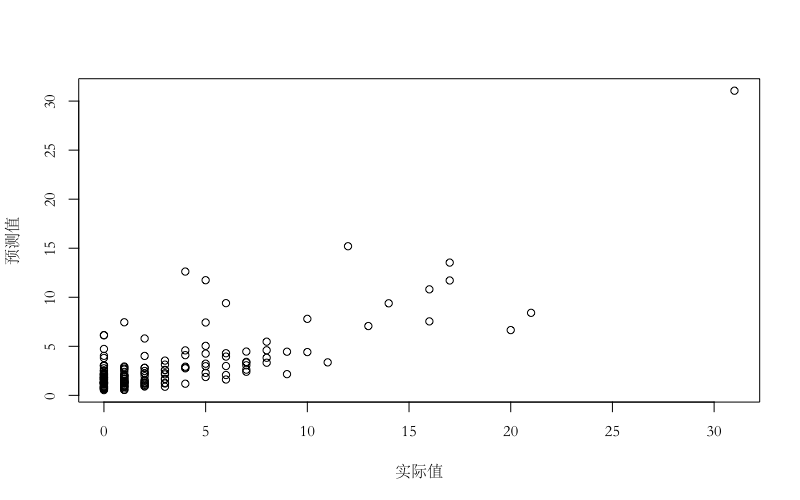
\includegraphics[width=300pt]{Rplot.png}
\caption{\small{lasso的预测结果}}
\end{figure}

\section{附录}

\subsection{因子载荷阵}

\begin{table}[H]
\centering
\caption{因子载荷阵}
\begin{tabular}{cccccccc}
  \hline
    字段 & 因子一 & 因子二 & 因子三 & 第四因子 & 第五因子 & 第六因子 & 共性方差 \\\hline
		年龄&-0.03 & 0.1 & 0.14 & -0.05 & 0.66 & -0.08 & 0.47 \\
		位置前锋 & 0.72 & -0.3 & 0.17 & 0.08 & 0.02 & 0.02 & 0.65 \\
		位置中场 & -0.24 & 0.11 & -0.81 & 0.07 & -0.07 & -0.09 & 0.74 \\
		出场 & 0.34 & 0.74 & 0.21 & 0.08 & 0.07 & -0.14 & 0.73 \\
		首发 & 0.24 & 0.83 & 0.28 & 0.07 & 0.1 & -0.08 & 0.84 \\
		出场时间 & 0.28 & 0.86 & 0.28 & 0.09 & 0.1 & 0.02 & 0.92 \\
		进球 & 0.89 & 0.1 & -0.12 & 0.07 & 0.29 & 0.15 & 0.93 \\
		助攻 & 0.53 & 0.38 & -0.3 & -0.38 & 0.03 & -0.05 & 0.66 \\
		传球 & 0.03 & 0.86 & -0.05 & -0.01 & 0.15 & 0.12 & 0.77 \\
		过人 & 0.54 & 0.36 & -0.32 & -0.19 & -0.26 & -0.16 & 0.66 \\
		抢断 & -0.23 & 0.81 & -0.02 & 0.15 & -0.08 & 0.24 & 0.8 \\
		越位 & 0.79 & -0.07 & -0.01 & 0.27 & 0.09 & -0.1 & 0.71 \\
		犯规 & 0.29 & 0.55 & 0.01 & 0.62 & -0.02 & 0.16 & 0.8 \\
		红牌 & -0.04 & 0.1 & -0.03 & 0.5 & -0.11 & -0.13 & 0.29 \\
		黄牌 & 0.11 & 0.51 & 0.22 & 0.45 & -0.2 & 0.39 & 0.72 \\
		射门 & 0.89 & 0.22 & -0.15 & 0.13 & 0.04 & 0.03 & 0.88 \\
		射正 & 0.91 & 0.14 & -0.12 & 0.11 & 0.12 & 0.03 & 0.9 \\
		射门成功率 & 0.19 & -0.02 & 0.09 & -0.15 & 0.71 & 0.17 & 0.59 \\
		头球进球 & 0.5 & 0.02 & 0.27 & 0.32 & 0.38 & -0.17 & 0.6 \\
		左脚进球 & 0.7 & 0.04 & -0.06 & -0.31 & 0.02 & 0.13 & 0.6 \\
		右脚进球 & 0.69 & 0.12 & -0.23 & 0.23 & 0.3 & 0.2 & 0.73 \\
		直接任意球进球 & 0.44 & 0.09 & 0 & -0.22 & -0.19 & 0.55 & 0.58 \\
		点球 & 0.28 & 0.18 & -0.24 & 0.24 & 0.46 & 0.45 & 0.63 \\
		赢得点球机会 & 0.72 & 0.02 & 0.08 & -0.17 & -0.19 & 0.1 & 0.6 \\
		拦截 & -0.31 & 0.78 & 0.24 & 0.07 & -0.05 & 0.19 & 0.8 \\
		解围 & -0.28 & 0.35 & 0.84 & 0.05 & 0.06 & 0.07 & 0.92 \\
		头球解围 & -0.25 & 0.32 & 0.85 & 0.07 & 0.07 & 0.06 & 0.9 \\
		后场解围 & -0.29 & 0.32 & 0.84 & 0.03 & 0.07 & 0.07 & 0.91 \\
		头球争顶成功 & 0.25 & 0.12 & 0.55 & 0.55 & 0.17 & -0.1 & 0.71 \\
		乌龙球 & -0.01 & 0.11 & 0.18 & -0.08 & 0.12 & 0.55 & 0.36 \\
    \hline
  \end{tabular}
\end{table}

\subsection{曼城和利物浦比较}

曼城和利物浦是英超联赛的两大豪门。在这两队中谁的球员比较强呢?我使用因子分析模型结合风玫瑰图对两队的前锋、中场和后卫球员进行了分别比较,比较的结果如下。

\begin{figure}[H]
\centering
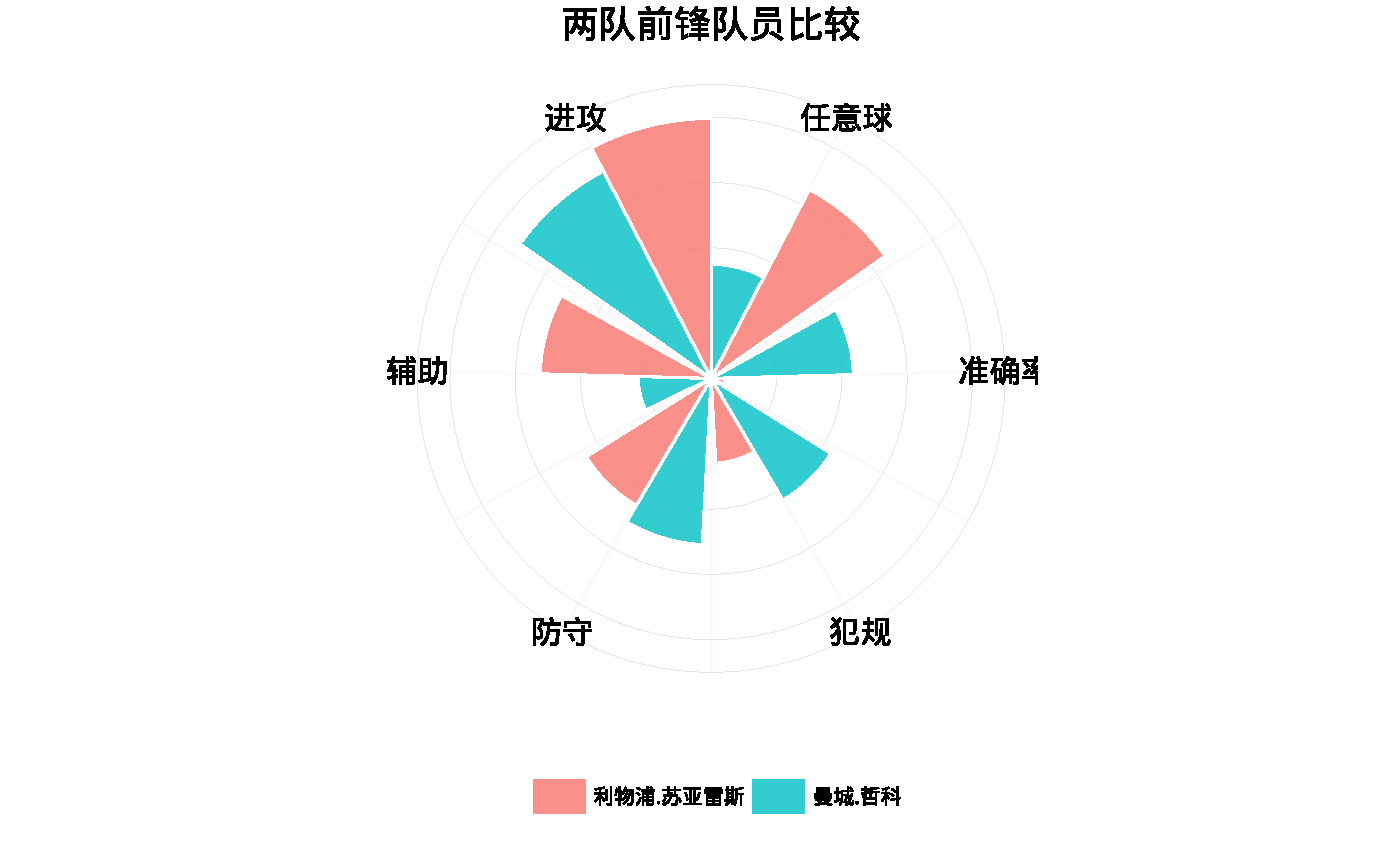
\includegraphics[width=133pt]{前锋94115.pdf}
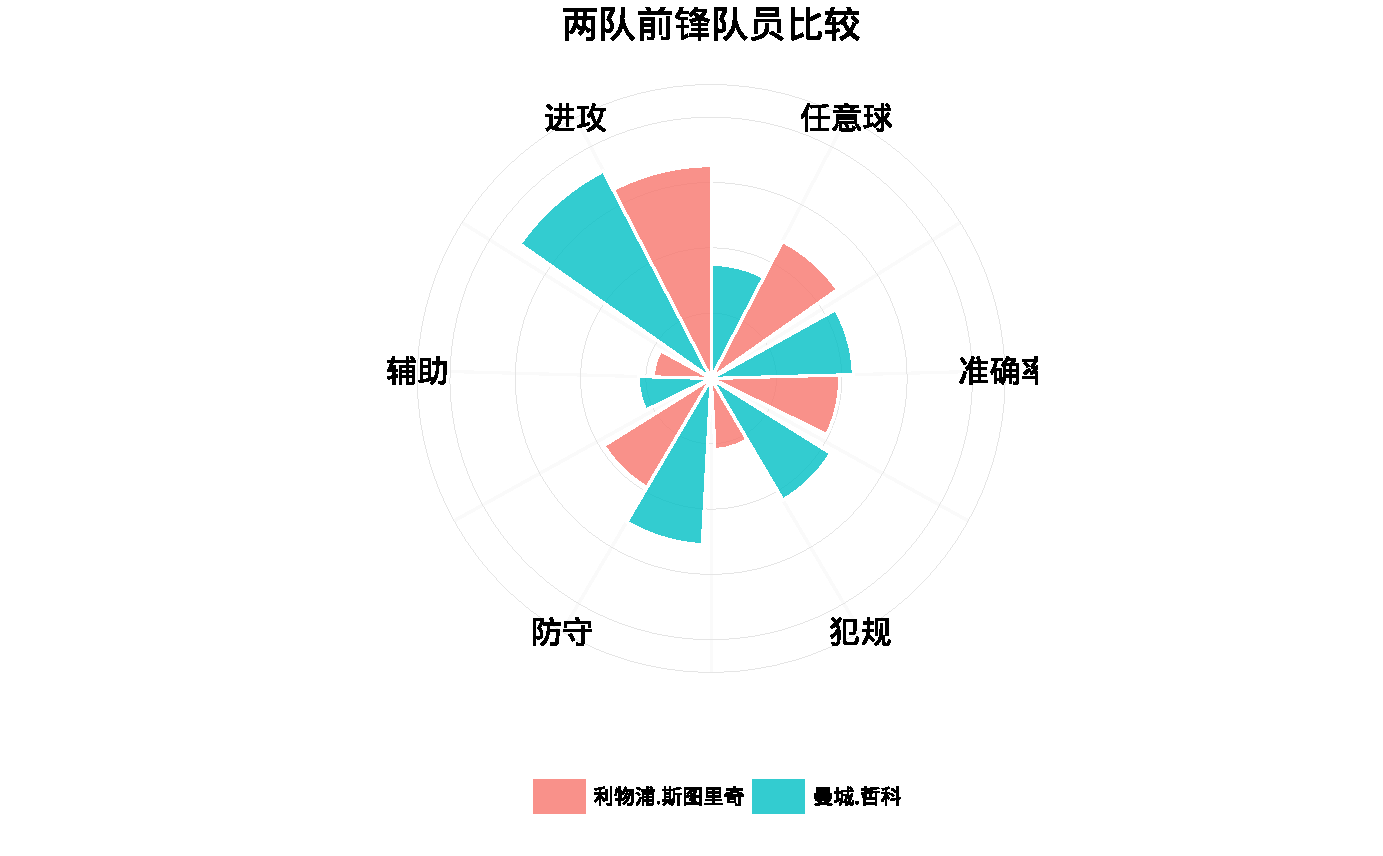
\includegraphics[width=133pt]{前锋94144.pdf}
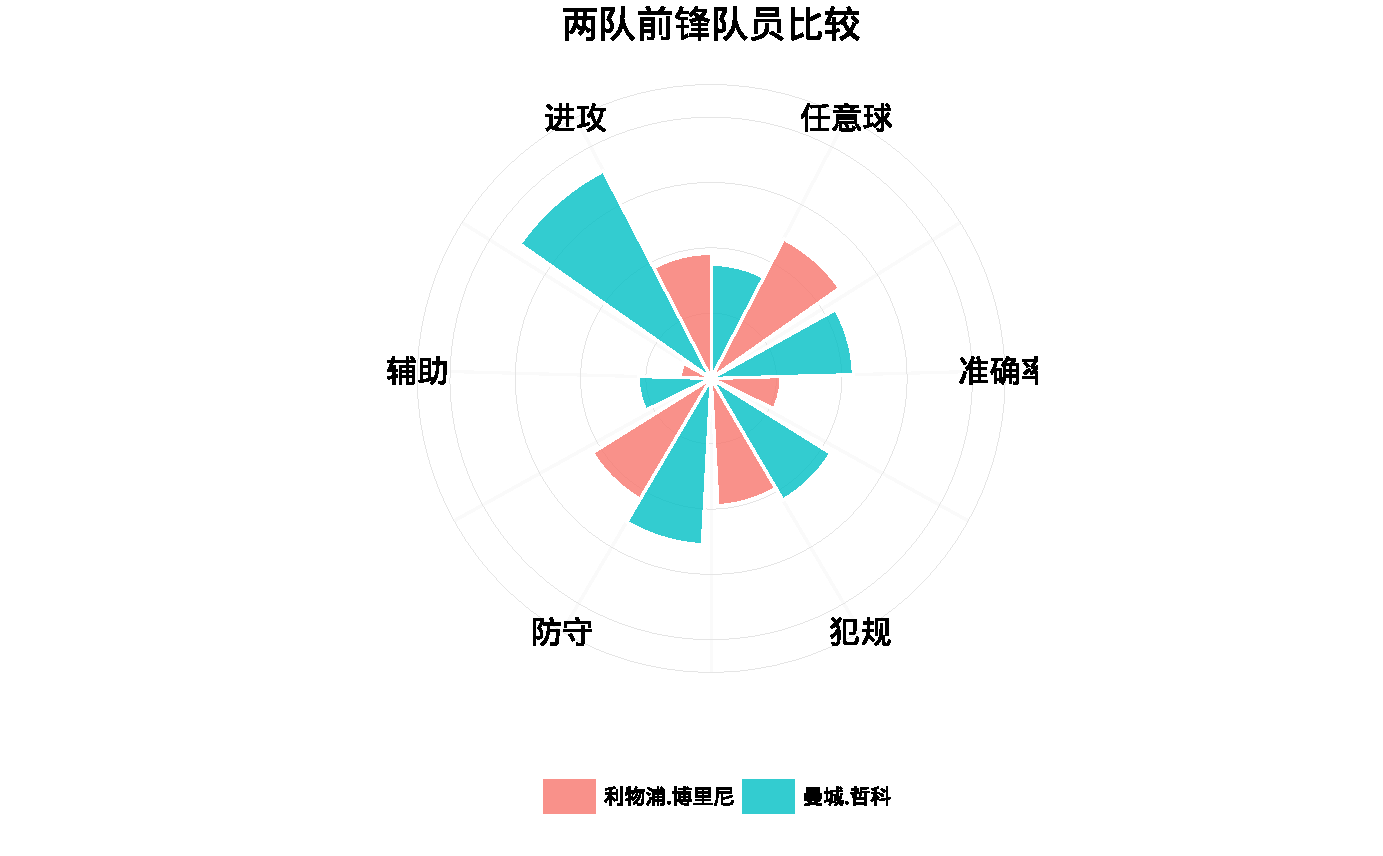
\includegraphics[width=133pt]{前锋94161.pdf}
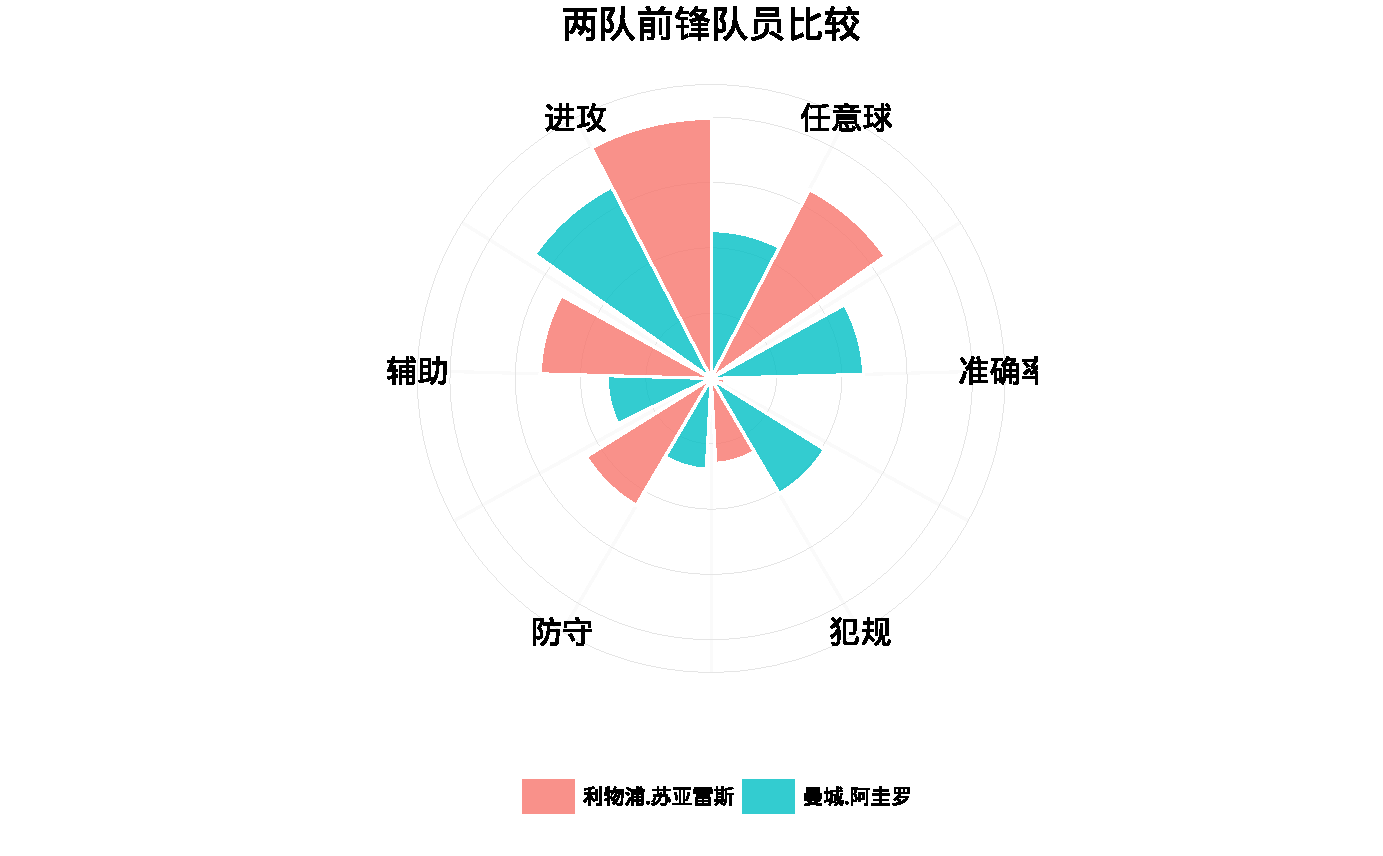
\includegraphics[width=133pt]{前锋128115.pdf}
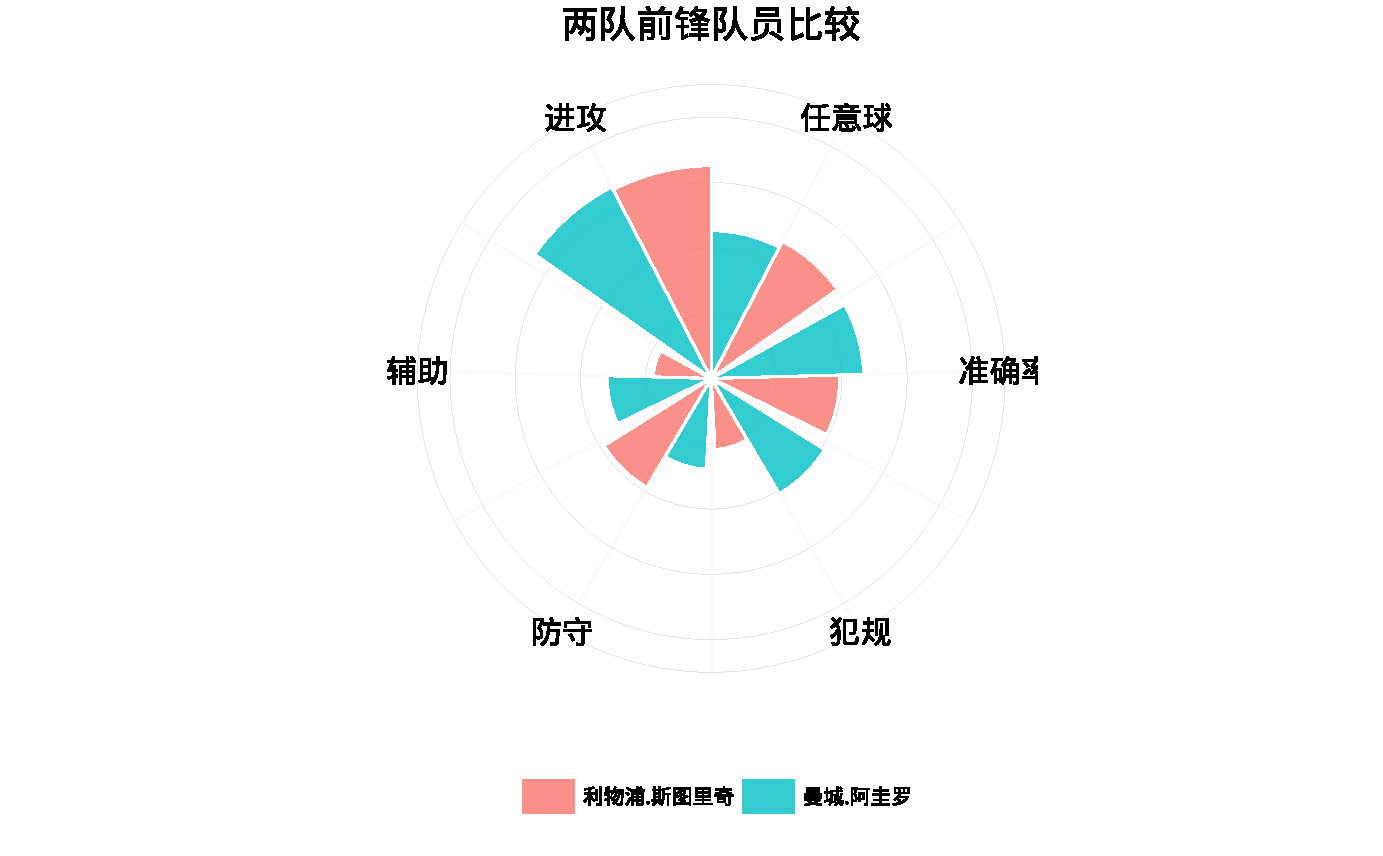
\includegraphics[width=133pt]{前锋128144.pdf}
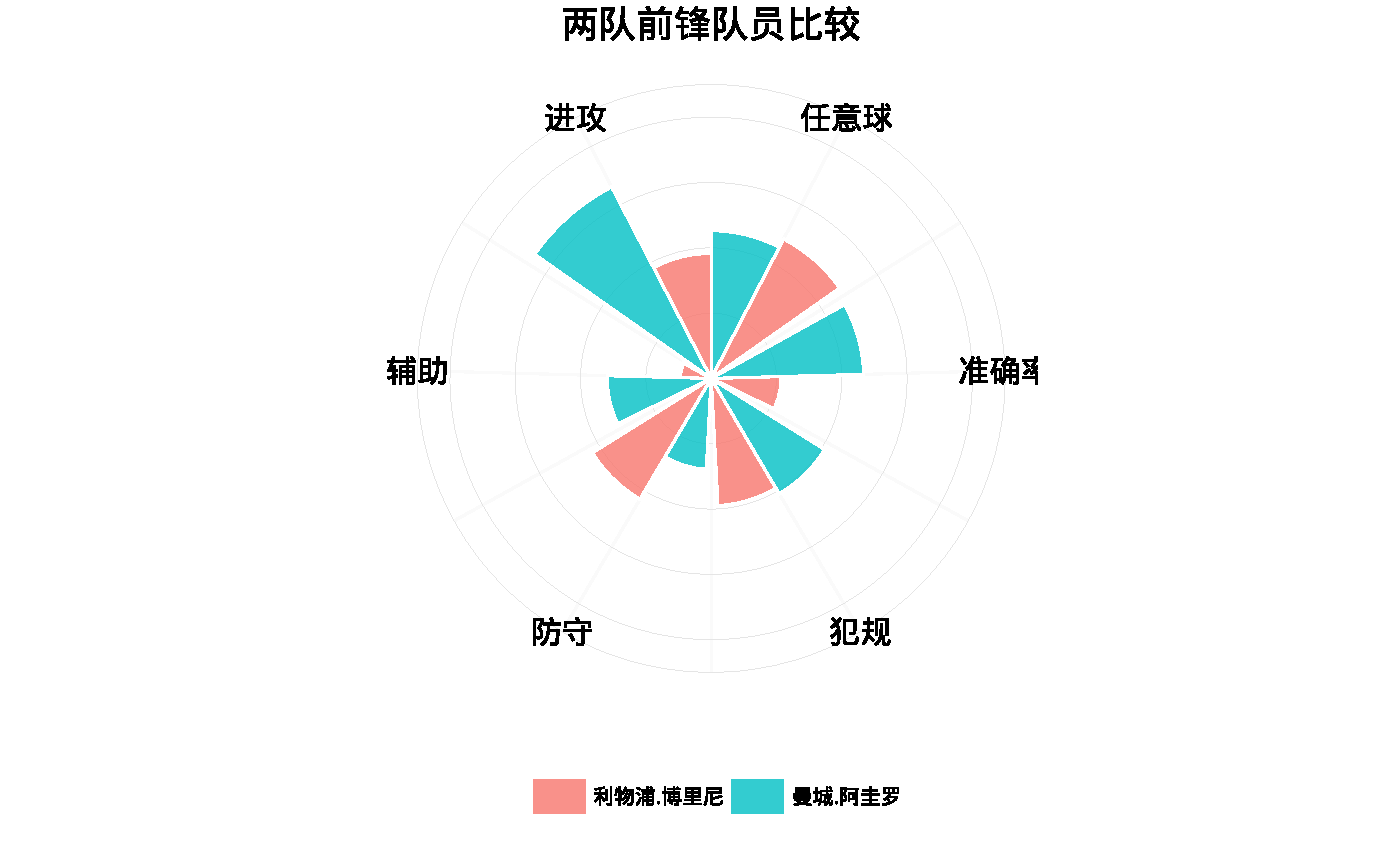
\includegraphics[width=133pt]{前锋128161.pdf}
\caption{\small{两队前锋比较}}
\end{figure}

从上图可以得出,尽管利物浦队的苏亚雷斯的进攻能力是最强的,但是利物浦对的另外两位前锋成绩却一般。曼城队的两位前锋虽然进攻能力比不上苏亚雷斯,但是他们的成绩比较平均且都好于曼城的另外两位前锋。

\begin{figure}[H]
\centering
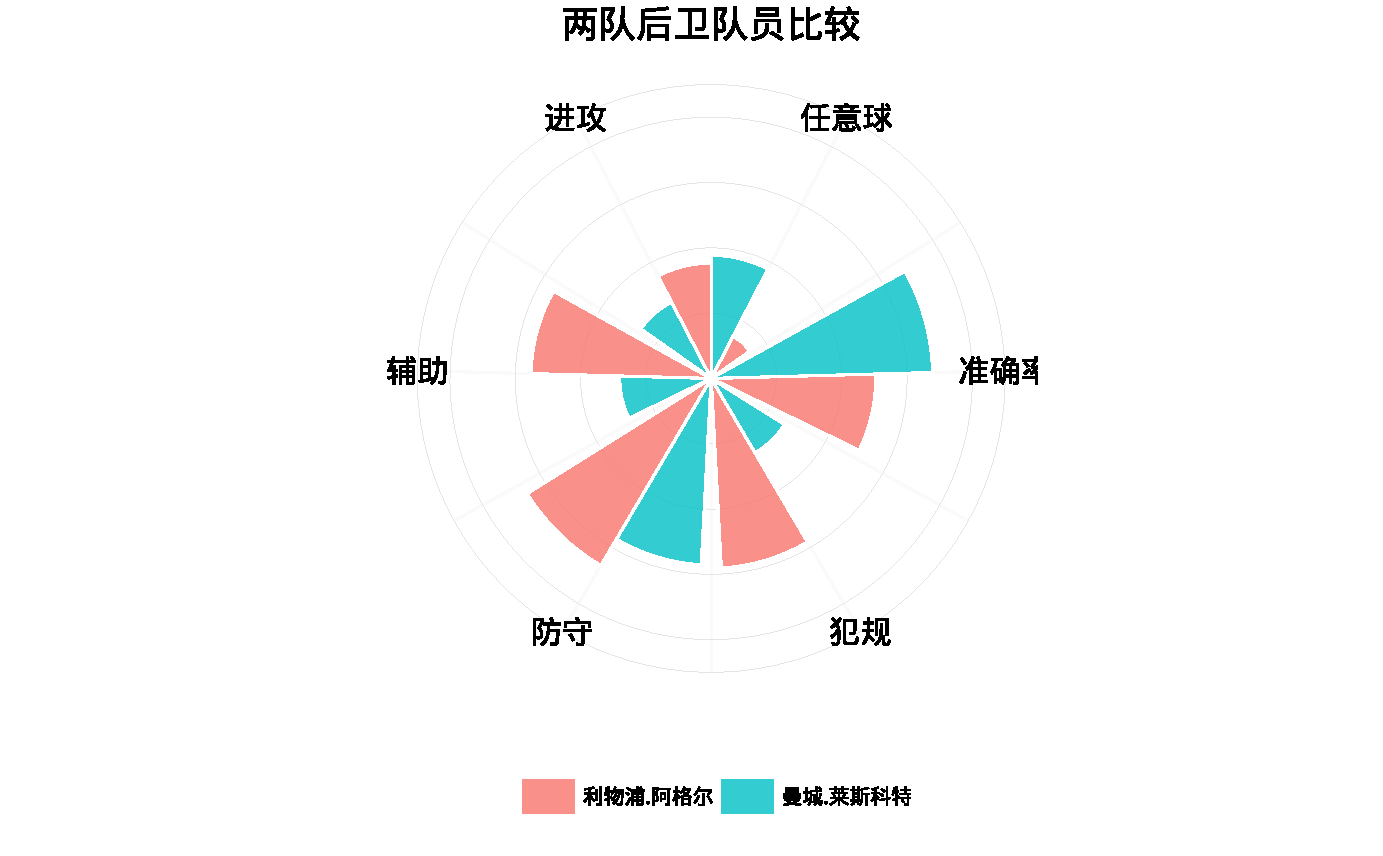
\includegraphics[width=100pt]{后卫2957.pdf}
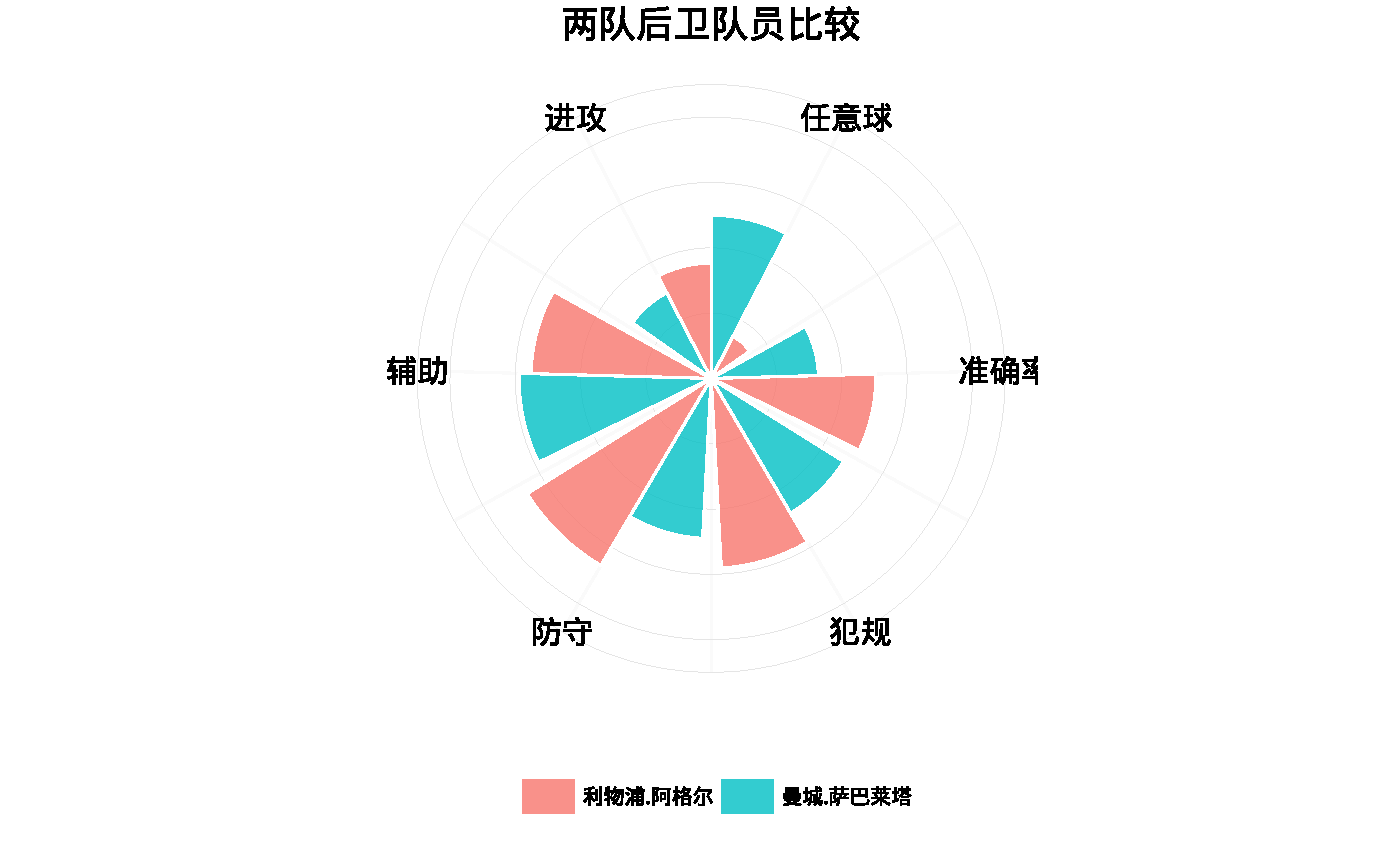
\includegraphics[width=100pt]{后卫7257.pdf}
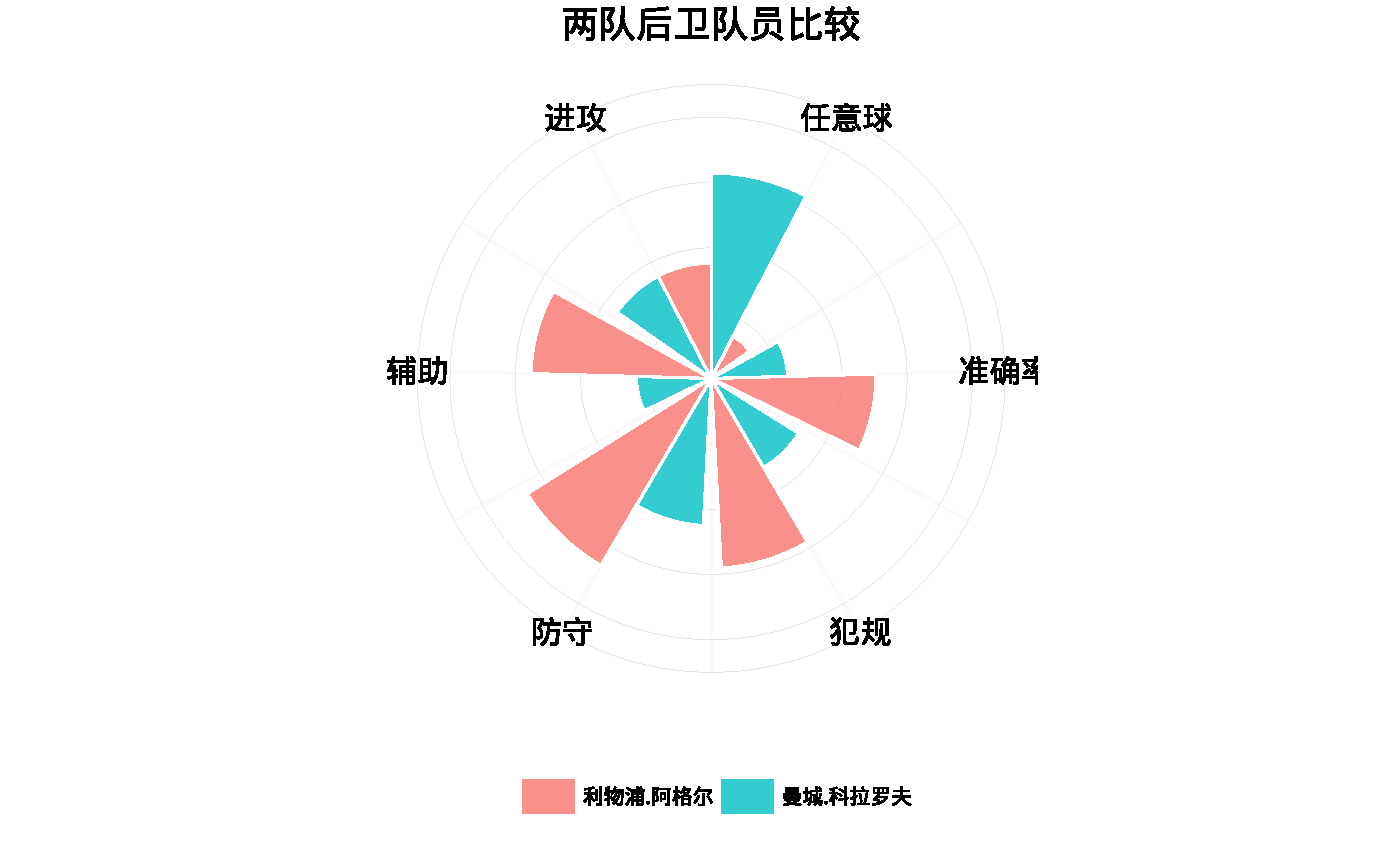
\includegraphics[width=100pt]{后卫7357.pdf}
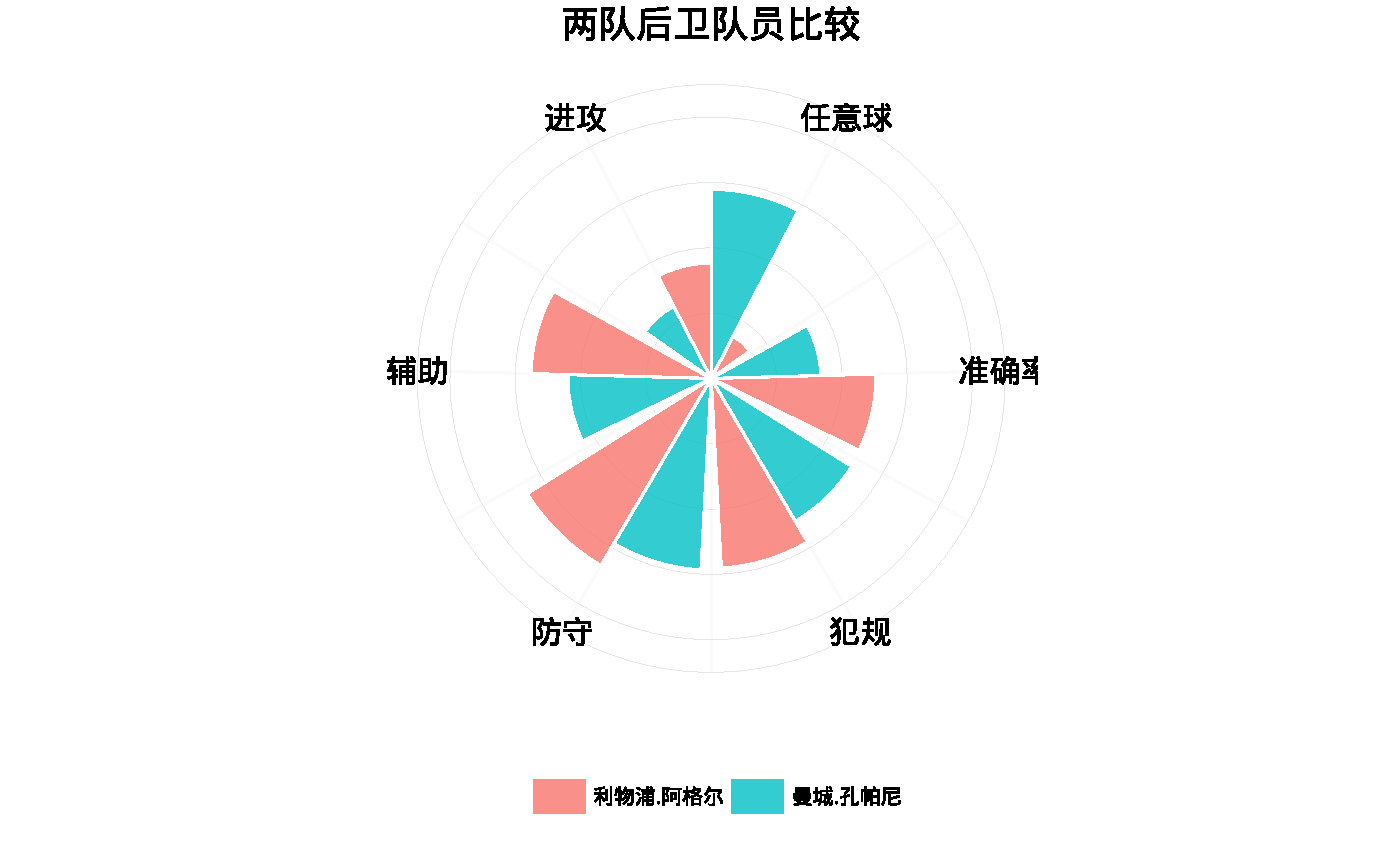
\includegraphics[width=100pt]{后卫9257.pdf}
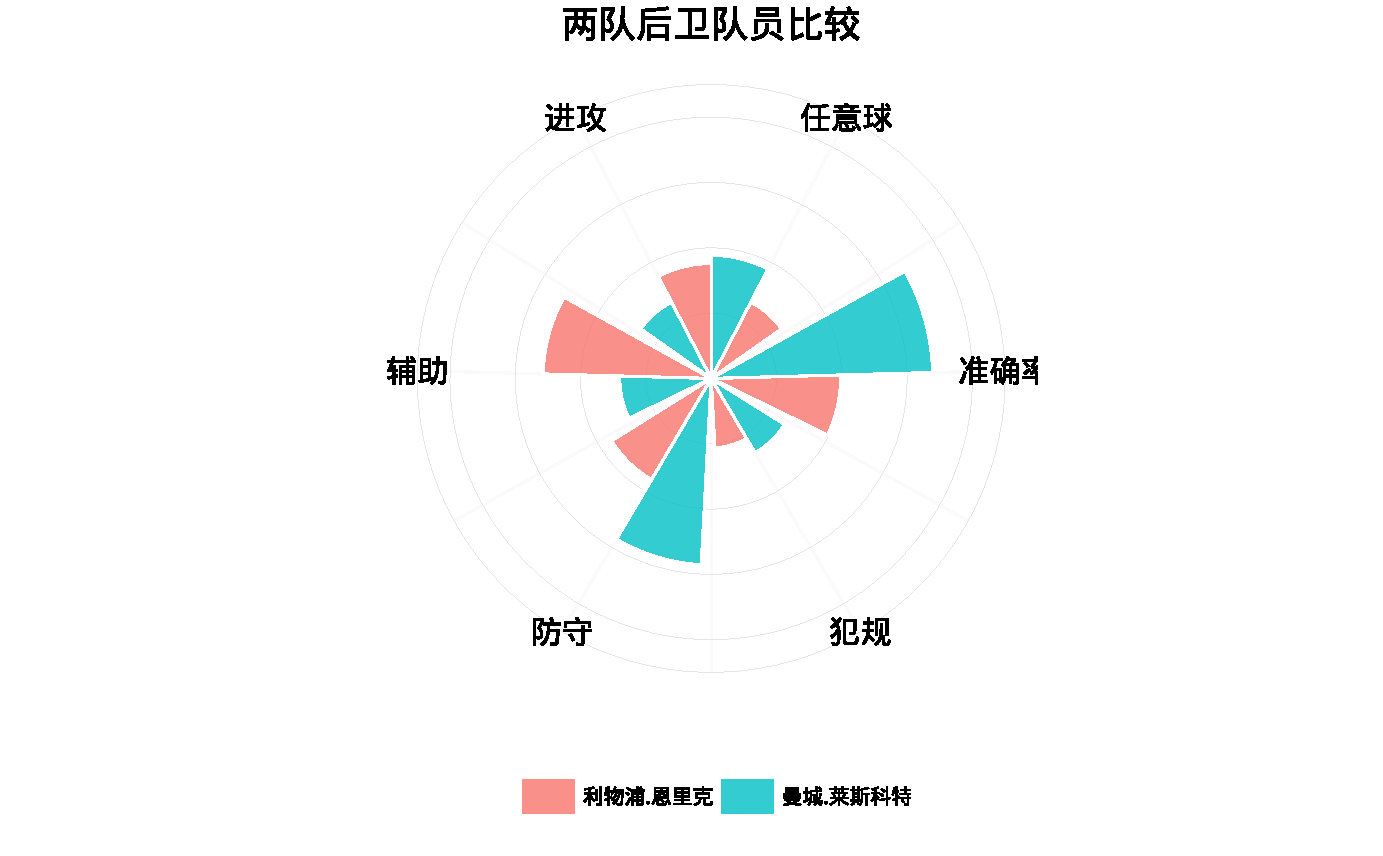
\includegraphics[width=100pt]{后卫2995.pdf}
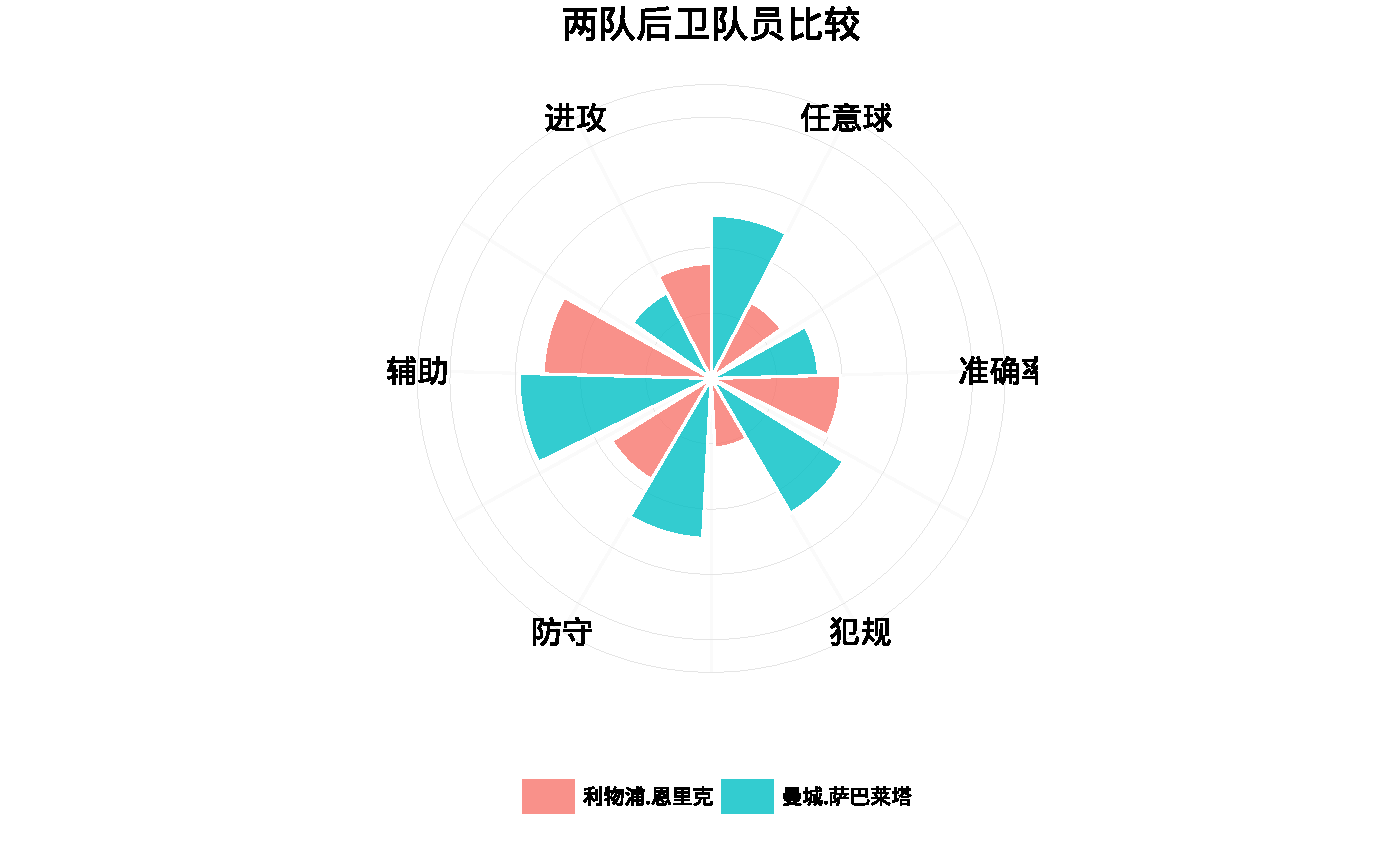
\includegraphics[width=100pt]{后卫7295.pdf}
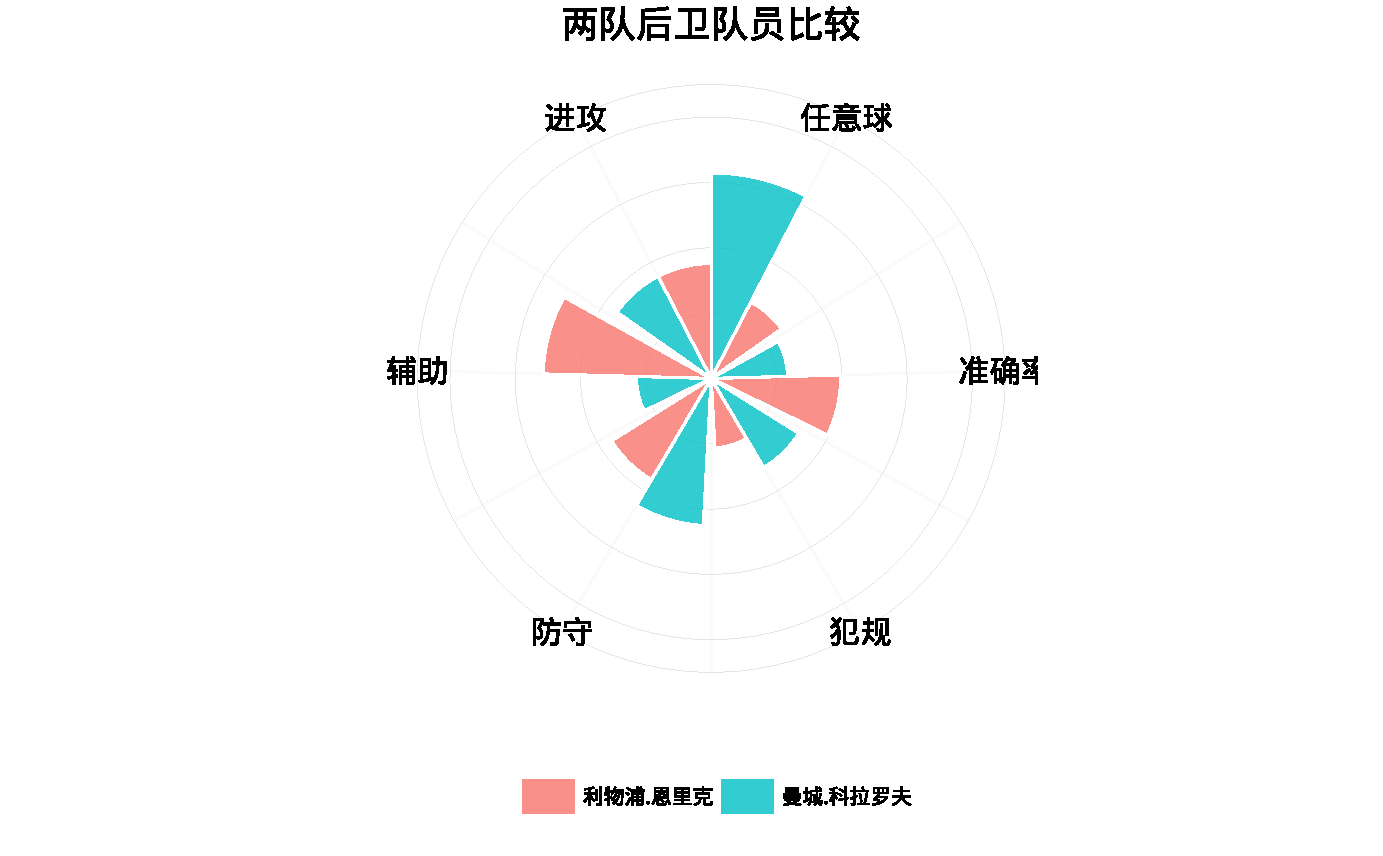
\includegraphics[width=100pt]{后卫7395.pdf}
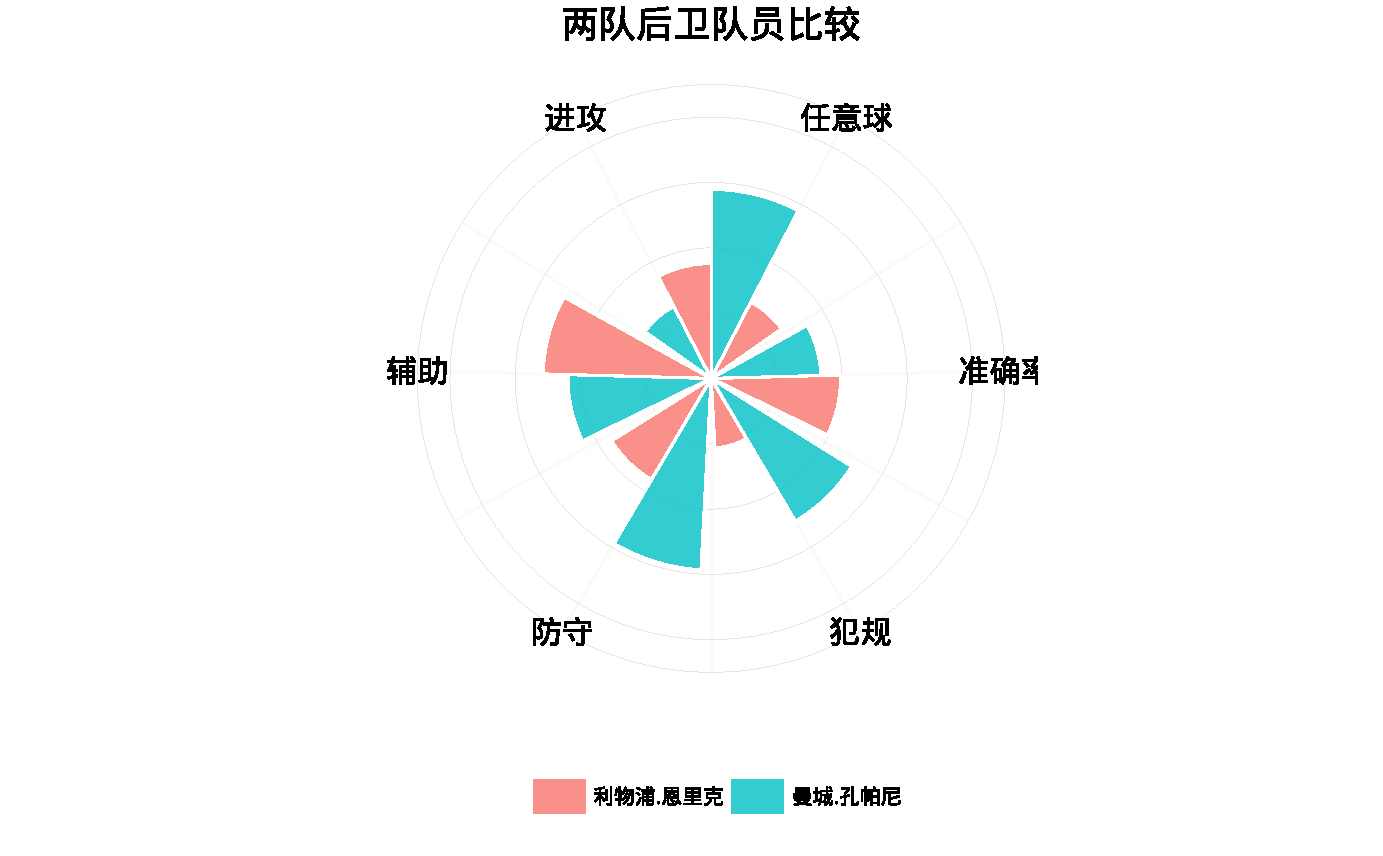
\includegraphics[width=100pt]{后卫9295.pdf}
\caption{\small{两队后卫比较}}
\end{figure}

两队的前锋和后卫哪家更强呢?相信在大家心中已经自有分晓。

\subsection{代码}

\lstinputlisting[language=R]{code.R}

\end{document}
